\documentclass[10pt,twocolumn]{article}

% Line spacing
\renewcommand{\baselinestretch}{1.05}
\widowpenalty=10000
\clubpenalty=10000
\hyphenpenalty=300
\tolerance=1000

% Packages
\usepackage[T1]{fontenc}
\usepackage{mathpazo}
\usepackage[scaled=0.9]{helvet}
\usepackage{courier}
\usepackage{microtype}
\usepackage{graphicx}
\usepackage{dblfloatfix}
\usepackage{adjustbox}
\usepackage{amsmath}
\usepackage{mathtools}
\usepackage{amsfonts}
\providecommand{\qed}{\hfill$\square$}
\usepackage{pifont}
\usepackage{amssymb}
\usepackage{booktabs}
\usepackage{tabularx}
\usepackage[table]{xcolor}
\usepackage{listings}
\PassOptionsToPackage{hyphens,spaces,obeyspaces}{url}
\usepackage[round,authoryear]{natbib}
\bibliographystyle{plainnat}
\usepackage{hyperref}
\usepackage{cleveref}
\usepackage{enumitem}
\usepackage{titlesec}
\usepackage{subcaption}
\usepackage{float}
\usepackage{placeins}
\usepackage{balance}
\usepackage[most]{tcolorbox}

% Caption styling
\usepackage{caption}
\captionsetup{font=small, labelfont=bf, labelsep=period, justification=justified, singlelinecheck=false, skip=8pt, belowskip=0pt}
\captionsetup[table]{position=top}
\setlength{\textfloatsep}{10pt plus 2pt minus 2pt}

% Section titles
\titleformat{\section}
  {\normalfont\Large\bfseries}{\thesection}{0.75em}{}
\titleformat{\subsection}
  {\normalfont\large\bfseries}{\thesubsection}{0.65em}{}
\titleformat{\subsubsection}
  {\normalfont\fontsize{11}{13}\selectfont\bfseries}{\thesubsubsection}{0.5em}{}
\titlespacing*{\section}{0pt}{0.8\baselineskip}{0.5\baselineskip}
\titlespacing*{\subsection}{0pt}{0.6\baselineskip}{0.4\baselineskip}
\titlespacing*{\subsubsection}{0pt}{0.5\baselineskip}{0.3\baselineskip}

% Page geometry
\usepackage[letterpaper, margin=1in]{geometry}
\usepackage{etoolbox}
\makeatletter
\patchcmd{\@maketitle}{\vskip 2em}{\vskip 0pt}{}{}
\makeatother

% Pin full-width floats to top
\makeatletter
\setlength{\@dblfptop}{0pt}
\setlength{\@dblfpbot}{0pt plus 1fil}
\makeatother

% Colors
\definecolor{harvardcrimson}{HTML}{A31F34}
\definecolor{codegreen}{HTML}{2D7A2D}
\definecolor{codegray}{HTML}{555555}
\definecolor{lightgray}{HTML}{F5F5F5}
\definecolor{napkinbg}{HTML}{FFF8E1}
\definecolor{napkinframe}{HTML}{C87B2A}
\definecolor{errorbg}{HTML}{FDE8E8}
\definecolor{errorframe}{HTML}{C44444}

\hypersetup{
  colorlinks=true,
  linkcolor=harvardcrimson,
  citecolor=blue,
  urlcolor=blue
}
\newcommand{\hrefurl}[2]{\href{#1}{\textcolor{blue}{#2}}}

% Napkin-math callout box (pedagogical worked examples)
\newtcolorbox{napkinmath}[1]{%
  enhanced,
  breakable,
  sharp corners,
  boxrule=0.8pt,
  colframe=napkinframe,
  colback=napkinbg,
  colbacktitle=napkinframe!15,
  coltitle=black!80,
  fonttitle=\small\bfseries\sffamily,
  title={Napkin Math: #1},
  toptitle=0.5ex,
  bottomtitle=0.5ex,
  left=0.8em,
  right=0.8em,
  top=0.6em,
  bottom=0.4em,
  before skip=\baselineskip,
  after skip=0.5\baselineskip,
  fontupper=\small,
}

% Error-case callout box (pedagogical failure examples)
\newtcolorbox{errorcase}[1]{%
  enhanced,
  breakable,
  sharp corners,
  boxrule=0.8pt,
  colframe=errorframe,
  colback=errorbg,
  colbacktitle=errorframe!15,
  coltitle=black!80,
  fonttitle=\small\bfseries\sffamily,
  title={Failure Case: #1},
  toptitle=0.5ex,
  bottomtitle=0.5ex,
  left=0.8em,
  right=0.8em,
  top=0.6em,
  bottom=0.4em,
  before skip=\baselineskip,
  after skip=0.5\baselineskip,
  fontupper=\small,
}

% Exercise callout box (structured classroom exercises)
\newtcolorbox{exercise}[1]{%
  enhanced,
  breakable,
  sharp corners,
  boxrule=0.8pt,
  colframe=harvardcrimson!70!black,
  colback=harvardcrimson!3,
  colbacktitle=harvardcrimson!12,
  coltitle=black!80,
  fonttitle=\small\bfseries\sffamily,
  title={Exercise: #1},
  toptitle=0.5ex,
  bottomtitle=0.5ex,
  left=0.8em,
  right=0.8em,
  top=0.6em,
  bottom=0.4em,
  before skip=\baselineskip,
  after skip=0.5\baselineskip,
  fontupper=\small,
}

% Code listing style
\lstset{
  basicstyle=\ttfamily\footnotesize,
  backgroundcolor=\color{lightgray},
  frame=single,
  rulecolor=\color{codegray},
  breaklines=true,
  showstringspaces=false,
  keywordstyle=\color{harvardcrimson}\bfseries,
  stringstyle=\color{codegreen},
  commentstyle=\color{codegray}\itshape,
  numbers=left,
  numberstyle=\scriptsize\color{codegray},
  xleftmargin=1.5em,
  framexleftmargin=1em,
  aboveskip=8pt,
  belowskip=6pt,
  language=Python
}

% Table body text
\newcommand{\tablebody}{\footnotesize}

% ============================================================================
% Computed Constants — single source of truth for inline math
% ============================================================================
\usepackage{pgfmath}
\newcommand{\cval}[1]{\pgfmathprintnumber[fixed, precision=1, 1000 sep={\,}]{#1}}
\newcommand{\cvalint}[1]{\pgfmathprintnumber[fixed, precision=0, 1000 sep={\,}]{#1}}

% --- Base hardware constants (H100 SXM datasheets) ---
\pgfmathsetmacro{\HhPeakTFLOPS}{989}
\pgfmathsetmacro{\HhBWTBs}{3.35}
\pgfmathsetmacro{\HhHBMGB}{80}
\pgfmathsetmacro{\NVLinkBWGBs}{900}
\pgfmathsetmacro{\IBBWGBs}{50}
\pgfmathsetmacro{\SRAMperSMKB}{228}

% --- Derived: Roofline ---
\pgfmathsetmacro{\HhRidgePoint}{\HhPeakTFLOPS / \HhBWTBs}

% --- Derived: Attention walkthrough ---
\pgfmathsetmacro{\SeqLen}{8192}
\pgfmathsetmacro{\HeadDim}{128}
\pgfmathsetmacro{\NumHeads}{32}
\newcommand{\AttnIntermMB}{128}       % 8192^2 * 2 / 1048576
\newcommand{\AttnTotalGB}{4}          % 128 * 32 / 1024
\pgfmathsetmacro{\TileSize}{256}
\newcommand{\TileKB}{128}  % 256*256*2/1024

% --- Model constants ---
\pgfmathsetmacro{\LLaMAParams}{70}
\pgfmathsetmacro{\LLaMAWeightsGB}{140}

% --- Derived: ZeRO ---
\pgfmathsetmacro{\ZeROMemGB}{1120}  % 140+140+840
\pgfmathsetmacro{\ZeROMinDevices}{14}  % ceil(1120/80)

% --- Derived: MoE ---
\pgfmathsetmacro{\MoEExperts}{16}
\pgfmathsetmacro{\MoEExpertGB}{8}
\pgfmathsetmacro{\MoETotalGB}{128}
\pgfmathsetmacro{\NVLinkIBgap}{\NVLinkBWGBs / \IBBWGBs}

% --- Edge-device constants (Apple M4 Pro, representative unified-memory SoC) ---
\pgfmathsetmacro{\EdgeRAMGB}{36}
\pgfmathsetmacro{\EdgeBWGBs}{273}
\pgfmathsetmacro{\EdgeTFLOPS}{53}
\newcommand{\EdgeCtxTokens}{1\,000\,000}
\newcommand{\EdgeCtxTokensRaw}{1000000}
\pgfmathsetmacro{\EdgeKVPerTokenMB}{0.5}
\newcommand{\EdgeKVTotalGB}{477}  % 0.5MB * 1M tokens / 1024

% --- Tensor parallelism constants ---
\pgfmathsetmacro{\TPdevices}{8}
\pgfmathsetmacro{\TPweightsPerDevice}{17.5}  % 140/8

\begin{document}

\title{
  \textbf{The Periodic Table of Machine Learning Systems}\\[0.3em]
  {\large A Constraint-Driven Design Heuristic with Compiler Correspondence}
}

\author{
  Vijay Janapa Reddi\\
  Harvard University
}

\date{\hrefurl{https://mlsysbook.ai}{mlsysbook.ai}}

\maketitle
\begingroup
\renewcommand{\thefootnote}{}%
\footnotetext{Part of the \emph{Machine Learning Systems} book ecosystem. Open-source tools: \url{https://github.com/mlsysbook/periodic-table}.}%
\endgroup

\begin{abstract}
Modern machine learning systems span from sub-milliwatt microcontrollers to multi-gigawatt datacenter fleets, yet practitioners learn the field as an unstructured catalog of branded techniques---FlashAttention, ZeRO, PagedAttention, Megatron-LM---each presented as a standalone invention. We argue that this catalog has a structure, and we make it explicit. We present \emph{The Periodic Table of Machine Learning Systems}: a design space of 90 primitives organized along eight abstraction layers (rows) and five information-processing roles (columns). Each element earns its place by satisfying a formal \emph{irreducibility criterion}---its performance cost cannot be expressed as a steady-state dataflow composition of same-layer components---which we prove constructively for irreducible cases (MAC units, Attention) and use to reject reducible composites (Systolic Arrays, Transformer Blocks).

To demonstrate that the table is generative rather than merely descriptive, we develop a \emph{Constraint-Driven Lowering Heuristic}: a four-filter search procedure that, given any physical constraint violation, prunes the table's 90 elements to a small set of candidate interventions---the same procedure a compiler uses to select a lowering pass. We validate the heuristic through five end-to-end walkthroughs (FlashAttention, ZeRO-3, PagedAttention, Megatron-LM tensor parallelism, and an unsolved million-token edge inference problem), each mechanically derived from a constraint violation with explicit napkin math, including a dead-end analysis that shows the heuristic pruning wrong paths before they consume engineering effort.

Three additional contributions ground the framework in established theory and practice. \emph{Molecular ML}, a compositional notation with seven operators, separates structural composition ($\otimes$, memory adjacency) from concurrent execution ($\parallel$, temporal overlap) and grounds its cost rules in the Roofline model with an explicit pipeline-bubble term. A \emph{generalized constraint operator} ($\mid_{C,\, p > \theta}$) extends the deterministic heuristic into the probabilistic regime where fleet-scale failures dominate. A \emph{structural correspondence to MLIR} maps each abstraction layer to a dialect level and each intervention to a graph rewrite rule expressed as a pattern-match-and-rewrite, with side-by-side \texttt{linalg}/\texttt{scf} code. Three ``Iron Law'' equations distill the framework into manipulable formulas for capacity, throughput, and serving efficiency. The result is an integrated framework for educators teaching ML systems, graduate students building transferable mental models, and engineers reasoning about hardware-software co-design.
\end{abstract}

\begin{figure*}[t!]
  \centering
  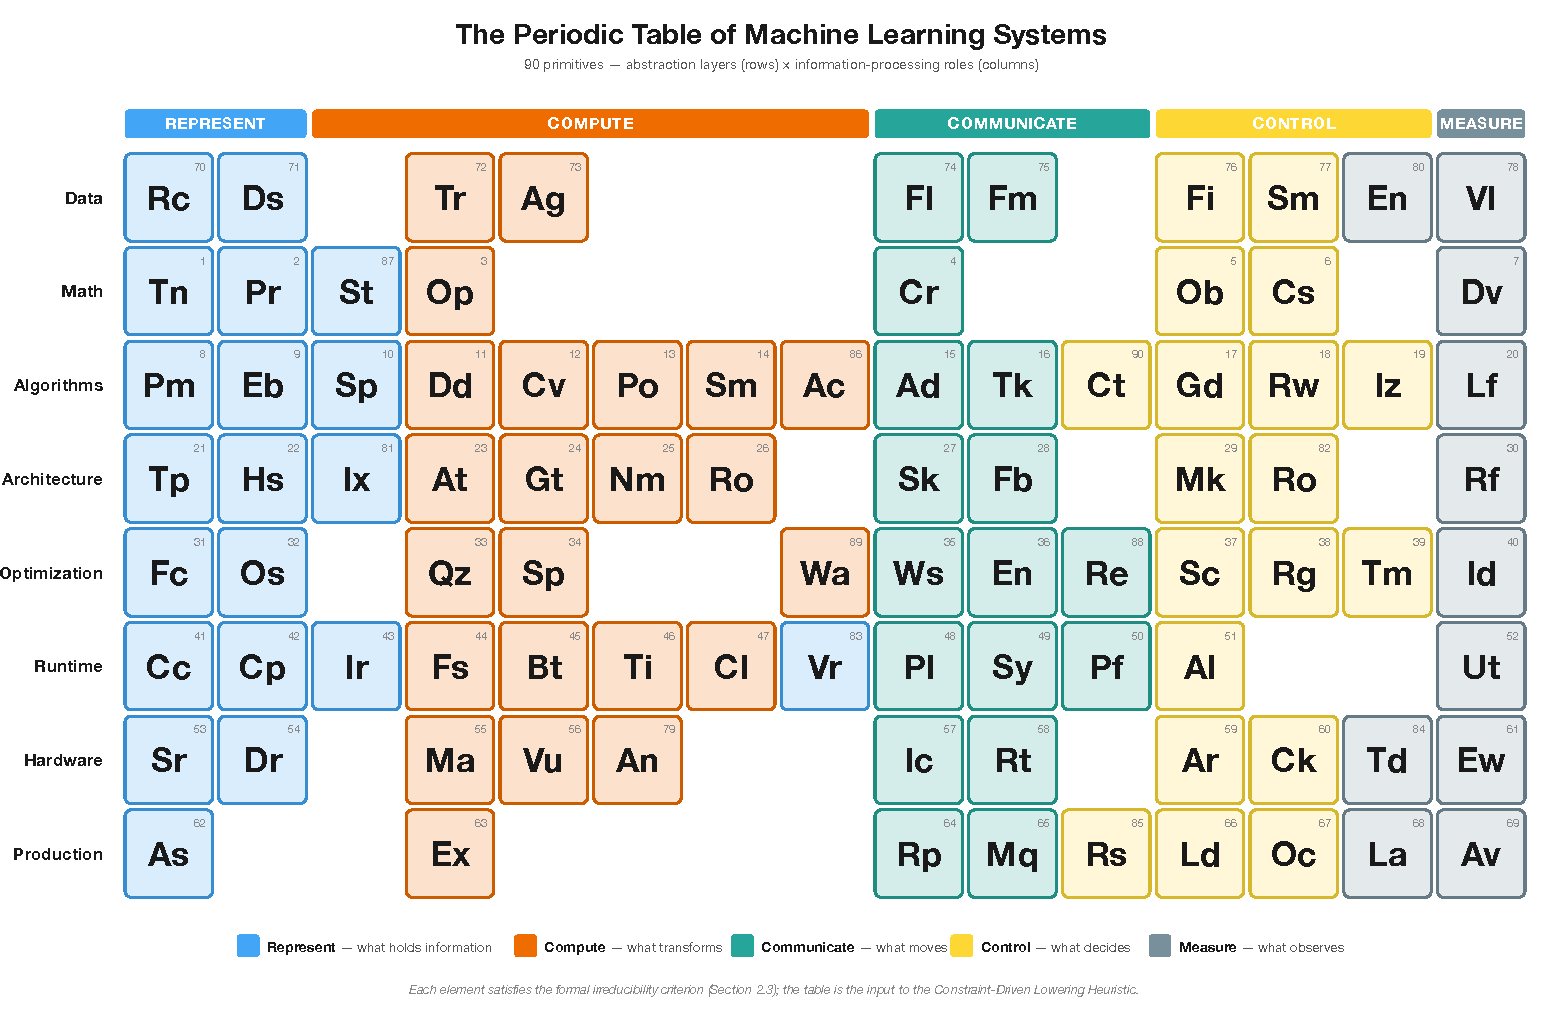
\includegraphics[width=\textwidth]{figures/periodic_table_hero.pdf}
  \caption{\textbf{The Periodic Table of Machine Learning Systems.} A design space of 90 primitives organized along eight abstraction layers (rows, Data through Production) and five information-processing roles (columns, Represent through Measure). Each element satisfies a formal irreducibility criterion (\Cref{sec:irreducibility}): its performance cost cannot be modeled at its own layer without lowering to the layer below. The table is the structured input that the Constraint-Driven Lowering Heuristic (\Cref{sec:resolution}) searches over---together they form an integrated framework for reasoning about ML systems. Color encodes role: blue for Represent, orange for Compute, teal for Communicate, yellow for Control, gray for Measure.}
  \label{fig:periodic-table}
\end{figure*}

% ============================================================================
\section{Introduction}
\label{sec:intro}

There is a fundamental tension at the heart of every machine learning system: the gap between high-level algorithmic intent and physical machine reality. A researcher writes \texttt{y = softmax(QK\textsuperscript{T}/$\sqrt{d}$)V} and expects attention. The hardware must materialize three matrices in HBM, stream them through a memory hierarchy with ${\sim}$\cval{\HhBWTBs}\,TB/s bandwidth, execute $O(n^2 d)$ multiply-accumulate operations on tensor cores, and write the result back---all within a latency budget that may be as tight as 10\,ms per token. When the sequence length doubles, the quadratic memory footprint exceeds the \cvalint{\HhHBMGB}\,GB HBM capacity of an H100, and a cascade of architectural decisions becomes inevitable: tiling, kernel fusion, sharding across devices, or some combination. The same pattern repeats across the field. Almost every advance in modern ML systems---FlashAttention for attention memory, ZeRO for distributed training memory, PagedAttention for serving fragmentation, Megatron-LM for cross-device weight capacity, continuous batching for arithmetic-intensity recovery---follows the same shape: a physical constraint binds, and an architectural intervention is the response. Yet the field is taught as a catalog of branded techniques, each presented as a standalone invention with a catchy name.

This paper argues that the catalog has a structure, and we make it explicit. We organize the field around \emph{The Periodic Table of Machine Learning Systems}, a design space of 90 primitives spanning eight abstraction layers (Data through Production) and five information-processing roles (Represent, Compute, Communicate, Control, Measure). Each element is admitted only if its performance cost cannot be modeled at its own layer---a formal irreducibility criterion that determines what counts as a primitive. Then, to demonstrate that the table is more than a labeling exercise, we develop a four-filter \emph{Constraint-Driven Lowering Heuristic} that searches the table mechanically: given any physical constraint violation, the filters prune the 90 elements to 1--3 candidate interventions, the same way a compiler pass selects a lowering rule. The combination is the contribution. The table by itself is a taxonomy; the heuristic by itself has nothing to operate on. Together they form a generative framework in which FlashAttention, ZeRO, PagedAttention, and Megatron-LM are not isolated inventions but the deterministic outputs of a structured search.

\paragraph{The thesis.} Modern ML systems are not a collection of clever tricks. They are a structured design space governed by physics, and the architectures that populate the field today are the deterministic consequences of physical constraint violations on specific hardware. Given the same constraint, the same hardware specifications, and a structured search over a bounded design space, any engineer arrives at the same architectural class. This paper provides both halves of that claim: the bounded design space (the Periodic Table) and the structured search (the constraint-driven heuristic).

\paragraph{Who will read this---and why.}

\emph{Educators} will use this paper to replace technique-by-technique instruction with constraint-driven derivation. The four-stage walkthroughs (\Cref{sec:walkthrough,sec:validation}), worked napkin-math examples (\Cref{sec:teaching}), and graph rewrite rules (\Cref{sec:grammar-formal}) provide a complete curriculum backbone. \emph{Graduate students} will use it as a Rosetta Stone: a unified framework that retroactively decodes five years of ML systems papers---each published with a catchy name as though it were a standalone paradigm---into instances of a single design pattern. The ``Predict the Paper'' exercise (\Cref{sec:predict-paper}) is the ultimate test: given only a constraint violation and hardware specifications, students derive the architecture of a published system before seeing its name. \emph{Production engineers} will use it as a diagnostic vocabulary: when a serving cluster's P99 latency spikes, the constraint operator and the four-filter search provide a structured triage---capacity, bandwidth, fragmentation, or straggler?---before reaching for a profiler. The framework's value to practitioners is not that it replaces cycle-accurate tools but that it narrows the search space \emph{before} instrumentation. If your system doesn't work at scale, you haven't defined the right primitives; the generalized constraint operator ($\mid_{C,\, p > \theta}$, \Cref{sec:probabilistic}) extends the deterministic heuristic into the probabilistic regime where fleet-scale failures dominate.

\paragraph{The value.} A taxonomy alone is cheap. What makes the Periodic Table valuable is not the labeling of 90 elements but the formal machinery that constrains \emph{which} elements deserve a place---the Irreducibility Criterion of \Cref{sec:irreducibility}---together with the search procedure that lets us derive systems from it: the Constraint-Driven Lowering Heuristic of \Cref{sec:resolution}, which makes the table generative. Around these two load-bearing pieces, the paper assembles the supporting machinery (cost rules, an MLIR correspondence, three Iron Laws) so that the framework can be used end-to-end---from a whiteboard sketch to a verified molecule to a compiler lowering pass. The full set of contributions is enumerated formally in the next paragraph, and \Cref{sec:taxonomy,sec:composition,sec:compiler,sec:walkthrough,sec:validation,sec:probabilistic,sec:teaching,sec:conclusion} develop them in order.

\paragraph{Scope.} The framework operates at the architectural design phase, providing a bounded search space for resolving physical constraint violations \emph{prior to implementation}. It provides order-of-magnitude cost estimation---sufficient to identify which constraint binds and what class of intervention is needed---within its explicit scope: deterministic, steady-state design on single nodes or small homogeneous clusters (\Cref{sec:composition}). It does \emph{not} replace cycle-accurate simulators, compiler IRs, or hardware profilers. The Molecular ML notation is analogous to big-$O$ for algorithms: useful for the \emph{first} design decision (memory-bound or compute-bound?), not for generating machine code. Beyond the single node, constraints become probabilistic: the constraint operator generalizes to $M \mid_{C,\, p > \theta}$, where $\theta$ is a design parameter balancing resilience cost against failure probability (\Cref{sec:probabilistic}).

\paragraph{The gap this paper fills.} The Roofline model \citep{williams2009roofline} characterizes individual kernels but is silent on cross-node architectures. MLIR \citep{lattner2021mlir} provides rigorous lowering semantics within a compilation unit but cannot express dataset ingestion rates or fleet reliability. The Berkeley 13 Dwarfs \citep{asanovic2006landscape} classified parallel motifs but did not represent hardware constraints. MLSysIM \citep{reddi2026mlsysim} formalizes ``Systems Walls'' as hard physical bounds but does not decompose systems into reusable primitives. Our framework complements these: the elements are the design-space dimensions, the walls are the constraints that prune infeasible compositions, and the lowering heuristic is the bridge between them. In \Cref{sec:compiler}, we show that this bridge has a precise structural correspondence to MLIR's own lowering mechanics.

\paragraph{Contributions.}

\begin{enumerate}[nosep, leftmargin=*, label=\textbf{C\arabic*.}]
\item \textbf{The Periodic Table of Machine Learning Systems with a formal irreducibility criterion.} A design space of 90 primitives organized along eight abstraction layers and five information-processing roles. Each element is admitted via a cost-model inequality over steady-state dataflow graphs that determines granularity with mathematical precision. We prove irreducibility for MAC units (tensor-core pipeline nonlinearity) and Attention ($O(n^2)$ intermediate memory) and prove \emph{reducibility} for Systolic Arrays (linear MAC composition) via a three-line derivation, demonstrating that the criterion can both admit and reject candidates (\Cref{sec:taxonomy,sec:irreducibility}).

\item \textbf{The Constraint-Driven Lowering Heuristic that makes the table generative.} Four filters operate as deterministic predicates over formalized element metadata (layer, role, constraint affinity, preconditions), pruning the table's 90 elements to 1--3 candidate interventions for any given constraint violation. The heuristic mechanizes the expert intuition that converts a constraint into an architecture; we validate it through five end-to-end walkthroughs---including a dead-end analysis showing pruned search branches---each with quantitative scratchpad work shown in full (\Cref{sec:resolution,sec:walkthrough,sec:validation}).

\item \textbf{Molecular ML: a compositional notation with Roofline-grounded cost semantics.} Seven operators with explicit separation of structural composition ($\otimes$, memory adjacency) from concurrent execution ($\parallel$, temporal overlap)---two algebraically distinct constructs that prior notations conflate. A pipeline-bubble term in the cost model captures the dominant inefficiency of multi-stage systems, and a generalized constraint operator ($\mid_{C,\, p > \theta}$) formalizes the boundary between deterministic and probabilistic regimes (\Cref{sec:composition,sec:probabilistic}).

\item \textbf{Structural correspondence to MLIR via DAG rewrite rules.} Each abstraction layer maps to an MLIR dialect level; each constraint-driven intervention maps to a graph transformation expressed as a pattern-match-and-rewrite on directed acyclic graphs. Side-by-side \texttt{linalg}/\texttt{scf} code demonstrates the mapping for FlashAttention's tiling and tensor parallelism's sharding---this is a concrete structural mapping, not an analogy (\Cref{sec:compiler,sec:grammar-formal}).
\end{enumerate}

\paragraph{Road map.} \Cref{sec:taxonomy} details the design space with a formalized irreducibility criterion including constructive proofs. \Cref{sec:composition} introduces Molecular ML with separated spatial/temporal operators, cost semantics including pipeline bubbles, and the four-filter heuristic. \Cref{sec:compiler} establishes the MLIR correspondence via DAG rewrite rules. \Cref{sec:walkthrough} provides a detailed FlashAttention walkthrough. \Cref{sec:validation} validates through four additional walkthroughs, including a dead-end analysis of million-token edge inference. \Cref{sec:probabilistic} formalizes the boundary between deterministic and probabilistic constraints. \Cref{sec:teaching} presents classroom tools, Iron Law equations, and exercises including a fleet-scale tail-at-scale problem. \Cref{sec:conclusion} addresses limitations and future directions.

% ============================================================================
\section{The Design Space: Structure and Axes}
\label{sec:taxonomy}

The Periodic Table (\Cref{fig:periodic-table}) is organized along two orthogonal axes: five columns representing information-processing roles and eight rows representing abstraction layers. Together they partition the field into 40 (layer, role) cells and populate those cells with 90 primitives---the design space that the rest of the paper builds on.

\paragraph{What ``periodic'' means here.} We use the word \emph{periodic} in a structural, not chemical, sense. The five role columns recur coherently across the eight abstraction-layer rows: every layer has a Represent, Compute, Communicate, Control, and Measure element, and elements sharing a role column interact with physical constraints in the same way regardless of the layer they inhabit. A Represent-role element resolves a capacity constraint at any layer; a Communicate-role element participates in bandwidth constraints at any layer. This is the periodicity claim---a regularity across layer/role pairs that lets reasoning about an element at one layer transfer to a sibling element in the same column. It is not an analogy to atomic number or electron configuration; it is a design-space symmetry that the Irreducibility Criterion (\Cref{sec:irreducibility}) makes precise.

\subsection{Columns: Information-Processing Roles}

Every element fulfills exactly one of five roles, derived from the von Neumann architecture's separation of storage, processing, communication, and control, augmented with observation:

\begin{enumerate}[nosep, leftmargin=*]
\item \textbf{Represent.} The encoding, storage, and structural persistence of information. At the Math layer: \texttt{Tensor (Tn)}, \texttt{Embedding (Eb)}. At the Hardware layer: \texttt{Register File (Rf)}, \texttt{SRAM (Sr)}, \texttt{HBM (Hb)}, \texttt{Host DRAM (Dr)}. This explicit enumeration of the memory hierarchy---absent from prior ML taxonomies---is essential because data movement between these levels dominates modern ML system performance \citep{jouppi2017datacenter,ivanov2021data}.

\item \textbf{Compute.} The transformation and mutation of information. At the Hardware layer: \texttt{MAC Unit (Ma)}, \texttt{Vector Unit (Vu)}, \texttt{Scalar Unit (Su)}. At the Algorithm layer: \texttt{Dense Dot (Dd)}, \texttt{Convolution (Cv)}. At the Runtime layer: \texttt{Kernel Fusion (Fs)}, \texttt{Tiling (Ti)}.

\item \textbf{Communicate.} The movement and routing of information across boundaries. At the Optimization layer: \texttt{Autodiff (Ad)}, \texttt{Sync/Collective (Sy)}. At the Hardware layer: \texttt{Interconnect (Ic)}, \texttt{NVLink (Nv)}, \texttt{PCIe (Pc)}. At the Production layer: \texttt{RPC Protocol (Rp)}.

\item \textbf{Control.} The governance of execution flow, resource allocation, and system behavior. At the Algorithm layer: \texttt{Objective (Ob)}, \texttt{Gating (Gt)}. At the Runtime layer: \texttt{Scheduler (Sc)}, \texttt{Orchestrator (Or)}.

\item \textbf{Measure.} The observation and quantification of system state \emph{without alteration}. At the Math layer: \texttt{Divergence (Dv)}, \texttt{Entropy (En)}. At the Hardware layer: \texttt{Latency (Lt)}, \texttt{Throughput (Tp)}, \texttt{Energy (Eg)}, \texttt{Memory Fragmentation (Fg)}. At the Production layer: \texttt{Stochastic Variance (Sv)}---the tail-latency and straggler distributions that dominate fleet-scale behavior (\Cref{sec:probabilistic}). These are the ``noble gases'' of the taxonomy: they characterize the system's physical state but do not participate in the computation.
\end{enumerate}

\subsection{Rows: Abstraction Layers}

The eight rows trace the lifecycle of information from raw data to production deployment:

\begin{enumerate}[nosep, leftmargin=*]
\item \textbf{Data.} Provenance, ingestion, and preparation: \texttt{Record (Rc)}, \texttt{Sample (Sp)}, \texttt{Stream (St)}, \texttt{Loader (Ld)}.
\item \textbf{Math.} The formal objects of computation: \texttt{Tensor (Tn)}, \texttt{Embedding (Eb)}, \texttt{Scalar (Sl)}, \texttt{Divergence (Dv)}.
\item \textbf{Algorithm.} Learned operations and building blocks: \texttt{Attention (At)}, \texttt{Dense Dot (Dd)}, \texttt{Convolution (Cv)}, \texttt{Gating (Gt)}.
\item \textbf{Architecture.} Structural composition: \texttt{Topology (Tp)}, \texttt{Residual (Rs)}, \texttt{Feedback (Fb)}, \texttt{Hidden State (Hs)}.
\item \textbf{Optimization.} Training-time strategies: \texttt{Autodiff (Ad)}, \texttt{Gradient Descent (Gd)}, \texttt{Factorization (Fc)}, \texttt{Quantization (Qz)}.
\item \textbf{Runtime.} Execution-time mechanisms: \texttt{Tiling (Ti)}, \texttt{Fusion (Fs)}, \texttt{Prefetching (Pf)}, \texttt{Caching (Cc)}, \texttt{Scheduler (Sc)}, \texttt{Virtualization (Vr)}.
\item \textbf{Hardware.} Physical resources: \texttt{MAC (Ma)}, \texttt{Vector Unit (Vu)}, \texttt{SRAM (Sr)}, \texttt{HBM (Hb)}, \texttt{Register File (Rf)}, \texttt{Interconnect (Ic)}.
\item \textbf{Production.} Deployment and lifecycle: \texttt{Artifact Store (As)}, \texttt{Load Balancer (Lb)}, \texttt{Canary (Cn)}, \texttt{Monitor (Mn)}, \texttt{Stochastic Variance (Sv)}.
\end{enumerate}

\paragraph{The memory hierarchy as a vertical story.} Each column tells a coherent vertical narrative. Consider Represent: information originates as a \texttt{Record} (Data), is formalized as a \texttt{Tensor} (Math), is learned as a \texttt{Parameter} (Algorithm), is structured via \texttt{Topology} (Architecture), is compressed via \texttt{Factorization} (Optimization), is materialized in \texttt{SRAM} or \texttt{HBM} (Hardware), and is persisted in an \texttt{Artifact Store} (Production). The Hardware layer distinguishes four levels---\texttt{Rf}, \texttt{Sr}, \texttt{Hb}, \texttt{Dr}---because data movement cost dominates arithmetic cost by orders of magnitude. A 32-bit floating-point multiply consumes ${\sim}$3.7\,pJ; reading the same operand from DRAM costs ${\sim}$640\,pJ, a 173$\times$ difference \citep{horowitz2014energy}. Any design space that abstracts away this hierarchy cannot explain why FlashAttention exists.

\subsection{Formal Irreducibility Criterion}
\label{sec:irreducibility}

The central design decision of any taxonomy is granularity. We formalize our resolution criterion as a cost inequality, with an explicit definition of the composing function $f$.

\paragraph{Definition.} An element $e$ at layer $L$ is \emph{irreducible} if there exists no decomposition $e = g(e_1, \ldots, e_k)$ where all $e_i$ reside at layer $L$ such that:
\begin{equation}
\label{eq:irreducibility}
\text{Cost}_L(e) = f\bigl(\text{Cost}_L(e_1), \ldots, \text{Cost}_L(e_k)\bigr)
\end{equation}
for any composing function $f$ drawn from the class of \emph{steady-state dataflow graphs}: directed acyclic graphs whose nodes are arithmetic operations ($+, \times, \max, \min$) over scalar cost metrics (throughput, latency, memory footprint) and whose edges carry data dependencies. That is, $f$ may be any polynomial, any piecewise-linear bound, or any DAG of such operations---the standard vocabulary of Roofline and bandwidth-delay models. If no such $f$ exists, accurately modeling $e$'s performance cost (within an order of magnitude) requires lowering to layer $L{-}1$.

This is a \emph{cost-model} criterion, not an implementation criterion. A MAC unit \emph{can} be decomposed into adders and multipliers at the circuit layer, but its cost at the Hardware layer---precision-dependent throughput (\cvalint{\HhPeakTFLOPS}\,TFLOP/s FP16 vs.\ 67\,TFLOP/s FP32 on the same chip)---cannot be derived from same-layer components. The $15\times$ gap is a property of the MAC's microarchitecture, not of its logical decomposition.\footnote{This parallels processor design: a RISC-V \texttt{ADD} is irreducible at the ISA layer even though it decomposes into carry-chain logic at the circuit layer. Every useful taxonomy chooses a resolution that matches its cost model.}

\paragraph{Proof of irreducibility: MAC Unit (Ma).} At the Hardware layer, let $\text{Ma} = g(\text{Adder}, \text{Multiplier})$. A dataflow-graph composition yields:
\begin{align}
\label{eq:mac-proof}
&f\bigl(\text{Cost}_L(\text{Adder}),\, \text{Cost}_L(\text{Multiplier})\bigr) \notag \\
&\quad = N_{\text{cores}} \cdot f_{\text{clk}} \cdot 2 \;\approx\; 67\;\text{TFLOP/s}.
\end{align}
But $\text{Cost}_L(\text{Ma}) = \cvalint{\HhPeakTFLOPS}\;\text{TFLOP/s}$ (FP16 tensor cores). The $14.8\times$ gap arises from the tensor-core pipeline's $4{\times}4{\times}4$ warp-level matrix multiply, a microarchitectural optimization invisible at the arithmetic level. Since $\cvalint{\HhPeakTFLOPS} \neq 67$ under any steady-state dataflow composition of adders and multipliers, the MAC is irreducible. \qed

\paragraph{Proof of irreducibility: Attention (At).} At the Algorithm layer, decompose attention into two Dense Dots and a Softmax: $\text{At} = g(\text{Dd}_1, \text{Sm}, \text{Dd}_2)$. Each component's cost is expressible independently: $\text{Cost}_L(\text{Dd}_i) = O(n \cdot d^2)$ FLOPs, $\text{Cost}_L(\text{Sm}) = O(n)$. But their \emph{composition} creates an $O(n^2 d)$ intermediate matrix $S = QK^T$ whose memory cost is a property of the attention \emph{pattern}, not of the individual matmuls:
\begin{equation}
\label{eq:attn-proof}
\text{Cost}_L(\text{At})_{\text{mem}} = O(n^2) \neq O(n d^2) + O(n) + O(n d^2)
\end{equation}
No dataflow graph over the individual costs recovers the quadratic memory term. Attention is irreducible. \qed

\paragraph{Proof of reducibility: Systolic Array.} A Systolic Array is a regular grid of $N \times N$ MAC units connected by nearest-neighbor links. Its cost decomposes as:
\begin{align}
\label{eq:systolic-proof}
\text{Throughput}(\text{SA}_{N \times N}) &= N^2 \times \text{Throughput}(\text{Ma}) \\
\text{Latency}(\text{SA}_{N \times N}) &= (2N - 1) \times \text{Latency}(\text{Ma}) \notag \\
\text{Energy}(\text{SA}_{N \times N}) &= N^2 \times \text{Energy}(\text{Ma}) + E_{\text{link}} \notag
\end{align}
where $E_{\text{link}}$ is the nearest-neighbor interconnect energy, itself a same-layer quantity. All three cost metrics are steady-state dataflow compositions of same-layer elements. The Systolic Array is \emph{reducible}: \Cref{eq:irreducibility} is satisfied, so it is rejected from the taxonomy. \qed

Similarly, a \emph{Transformer Block} is reducible: its cost decomposes into independently modelable attention and feed-forward components at the same layer.

\paragraph{The boundary of irreducibility.} The key distinction is \emph{emergent cost}---cost that arises from the interaction of components in a way that no DAG over individual component costs can predict. Tensor cores exhibit emergent throughput (pipeline scheduling). Attention exhibits emergent memory (quadratic intermediate). Systolic arrays do not: their cost scales linearly and predictably from their constituents. This boundary is mathematically airtight because the class of composing functions $f$ is precisely defined.

% ============================================================================
\section{Molecular ML: A Compositional Notation}
\label{sec:composition}

The Periodic Table tells us \emph{which} primitives exist; Molecular ML tells us how to \emph{compose} them. Production ML systems are not isolated elements but structured molecules---assemblies of multiple primitives bound by data dependencies, memory adjacency, and concurrent execution, all subject to physical constraints. To reason about such molecules quantitatively, we define \emph{Molecular ML}: a compositional notation with seven operators (the critical separation being structural composition $\otimes$ from concurrent execution $\parallel$), Roofline-grounded cost semantics with an explicit pipeline-bubble term, and constraint-driven design heuristics that turn the notation into a search procedure.

\paragraph{Scope and applicability.} Molecular ML is a \emph{deterministic, steady-state} design language. Its cost rules assume uniform hardware, static constraint bounds, and synchronous execution. This makes it accurate within a single node or a small homogeneous cluster ($\leq$64 devices on uniform interconnect), and progressively less accurate as fleet size, topological non-uniformity, and probabilistic failure modes dominate. At 1,024+ GPUs, the probability that at least one node experiences a transient slowdown per training step exceeds 70\%. Rather than treating this as a late limitation, we introduce the \emph{generalized constraint operator} here:
\begin{equation}
\label{eq:gen-constraint}
M \;\mid_{C,\; p > \theta}
\end{equation}
For deterministic constraints (single-node), $\theta = 0$: any violation triggers search. For probabilistic constraints (fleet-scale), $\theta \in (0, 1)$ is a design parameter balancing resilience cost against failure probability. The deterministic case ($\theta = 0$) governs the remainder of this section; \Cref{sec:probabilistic} develops the probabilistic extension.

We emphasize what Molecular ML \emph{is}: a structured shorthand for whiteboard reasoning, analogous to big-$O$ notation for algorithms. Big-$O$ does not generate optimal code, but it tells you whether your algorithm is $O(n \log n)$ or $O(n^2)$. Similarly, Molecular ML does not generate optimal kernels, but it tells you whether your system is memory-bound or compute-bound and which class of intervention resolves the bottleneck---the first decision in system design.

\subsection{Visual Representation: Thinking in Block Diagrams}
\label{sec:visual}

Computer architects and systems engineers think in block diagrams, Rooflines, and dependency graphs---not in linear algebraic strings. The \emph{primary} representation of a Molecular ML compound is therefore a colored block diagram (\Cref{fig:flashattn}), where each element is drawn as a box colored by its Periodic Table role (blue for Represent, green for Compute, orange for Communicate, red for Control), with arrows showing dataflow and memory-residency annotations shown as background regions. Constraints are drawn as red boundary lines that the molecule must fit within.

The linear string notation defined below is the \emph{secondary} representation: a compact textual encoding for use in prose, code comments, and the constraint checker. It exists to make molecules writable in running text and parseable by tools. Every molecular formula should be read alongside its visual diagram.

\subsection{The Seven Operators}

\Cref{tab:operators} defines the seven operators. The critical design decision is the separation of \emph{structural composition} ($\otimes$) from \emph{concurrent execution} ($\parallel$)---two fundamentally different algebraic constructs that prior notations conflate.

\begin{table}[ht]
\tablebody
\centering
\caption{\textbf{Molecular ML operators.} Seven operators with formal cost interactions. $\otimes$ and $\parallel$ are algebraically distinct: the former sums memory (capacity), the latter takes the max of time (latency).}
\label{tab:operators}
\begin{tabularx}{\columnwidth}{@{} c l X @{}}
\toprule
\textbf{Op} & \textbf{Name} & \textbf{Semantics} \\
\midrule
$\rightarrow$ & Sequence & Output of left feeds input of right. \\
$\otimes$ & Adjacency & Structural co-residence in memory; sums capacity. \\
$\parallel$ & Concurrency & Temporal overlap of execution; max of time. \\
$[\cdot]^N$ & Repeat & Iterative replication $N$ times. \\
$\langle \cdot \rangle_{\text{mem}}$ & Residency & Data resides at memory level \emph{mem}. \\
$\mid_C$ & Constraint & Physical bound $C$; triggers search on violation. \\
$\xrightarrow{\text{bw}}$ & Transfer & Data movement at bandwidth \emph{bw}. \\
\bottomrule
\end{tabularx}
\end{table}

\paragraph{Why two composition operators.} Spatial composition and temporal composition are algebraically incompatible. Adjacency ($\otimes$) is commutative and associative over \emph{memory}: $\text{mem}(A \otimes B) = \text{mem}(A) + \text{mem}(B)$. Concurrency ($\parallel$) is commutative and associative over \emph{time}: $T(A \parallel B) = \max(T_A, T_B)$. Overloading a single $\parallel$ operator for both creates ambiguity in any graph representation: does $Q \parallel K$ mean ``$Q$ and $K$ reside simultaneously'' (a capacity claim) or ``$Q$ and $K$ execute concurrently'' (a latency claim)? In prior notations, disambiguation required inspecting the operand's semantic role. We eliminate this ambiguity structurally:

\begin{itemize}[nosep, leftmargin=*]
\item \textbf{Adjacency ($\otimes$):} $Q \otimes K \otimes V$ means all three tensors must reside simultaneously in the same memory level. This is a \emph{capacity} statement. Cost: $\text{mem}(Q \otimes K \otimes V) = \text{mem}(Q) + \text{mem}(K) + \text{mem}(V)$.

\item \textbf{Concurrency ($\parallel$):} $\text{Pf} \parallel \text{Vu}$ means prefetching layer $\ell{+}1$ runs concurrently with compute on layer $\ell$. This is a \emph{latency} statement. Cost: $T(\text{Pf} \parallel \text{Vu}) = \max(T_{\text{Pf}}, T_{\text{Vu}})$.
\end{itemize}

\paragraph{Operator semantics.} Sequence ($\rightarrow$) is not commutative: $A \rightarrow B$ means $A$'s output feeds $B$'s input, and their execution is ordered. Residency ($\langle \cdot \rangle_{\text{mem}}$) is an annotation that pins data to a specific memory level (\texttt{Rf}, \texttt{Sr}, \texttt{Hb}, \texttt{Dr}, or \texttt{Net}). Constraint ($\mid_C$) is a predicate that evaluates to \emph{satisfied} or \emph{violated}; when $\theta > 0$, it evaluates to \emph{violated with probability $p > \theta$}.

\paragraph{Example molecule.} Standard attention:
\begin{equation}
\label{eq:naive}
M_{\text{naive}} = (Q \otimes K \otimes V) \rightarrow Dd \rightarrow \text{Sm} \rightarrow Dd
\end{equation}

\subsection{Cost Semantics: How Operators Interact with Physics}
\label{sec:cost-model}

Each operator interacts with physical constraints according to five rules, grounded in the Roofline model \citep{williams2009roofline}.

\paragraph{The Roofline in one equation.} Every molecular formula implicitly defines an arithmetic intensity $I$ (FLOP/byte transferred):
\begin{equation}
\label{eq:roofline}
\text{Perf}(I) = \min\!\left(\underbrace{\pi}_{\text{peak FLOP/s}},\;\; \underbrace{\beta \cdot I}_{\text{bandwidth ceiling}}\right)
\end{equation}
where $\pi$ is peak compute (e.g., \cvalint{\HhPeakTFLOPS}\,TFLOP/s for H100 FP16) and $\beta$ is peak memory bandwidth (e.g., \cval{\HhBWTBs}\,TB/s for H100 HBM). The \emph{ridge point}:
\begin{equation}
\label{eq:ridge}
I^{*} = \frac{\pi}{\beta} = \frac{\cvalint{\HhPeakTFLOPS} \times 10^{12}}{\cval{\HhBWTBs} \times 10^{12}} \approx 295 \;\text{FLOP/byte}
\end{equation}

If $I < I^{*}$, the molecule is \emph{memory-bandwidth-bound}; if $I > I^{*}$, \emph{compute-bound}. This single number determines the optimization strategy.

\paragraph{Rule 1: Adjacency sums memory.}
\begin{equation}
\label{eq:parallel-mem}
\text{mem}(A \otimes B) = \text{mem}(A) + \text{mem}(B)
\end{equation}
This is a capacity claim: $A$ and $B$ must reside simultaneously.

\paragraph{Rule 2: Concurrency takes the maximum time.}
\begin{equation}
\label{eq:concurrent-time}
T(A \parallel B) = \max(T_A,\; T_B) + \delta_{\text{bubble}}
\end{equation}
where $\delta_{\text{bubble}}$ is the \emph{concurrency bubble}---the startup and drain overhead of pipelining two stages. For a $p$-stage pipeline with microbatch size $m$:
\begin{equation}
\label{eq:bubble}
\delta_{\text{bubble}} = \frac{p - 1}{p - 1 + m} \cdot T_{\text{total}}
\end{equation}
This term is the primary driver of systems like GPipe and PipeDream: at $p = 4$ stages, achieving $<10\%$ bubble fraction requires $m \geq 27$ microbatches. Omitting this term---as simpler notations do---makes pipeline parallelism appear free, which is why students consistently underestimate its overhead.

\paragraph{Rule 3: Sequential composition chains bandwidth.} If $A \rightarrow B$ and the output of $A$ must move from memory level $m_1$ to $m_2$:
\begin{equation}
\label{eq:seq-bw}
T_{\text{transfer}}(A \rightarrow B) = \frac{|\text{output}(A)|}{\text{bw}(m_1 \to m_2)}
\end{equation}
Total time is $\max(T_{\text{compute}},\; T_{\text{transfer}})$ when pipelining is possible.

\paragraph{Rule 4: Repeat multiplies cost; tiling amortizes it.} Applying $[\cdot]^N$ multiplies compute by $N$. Combined with a residency change---$[Ti \rightarrow (\cdot)_{\langle \text{Sr} \rangle}]^{N/B}$---memory per iteration drops from $O(N)$ to $O(B)$, and effective arithmetic intensity \emph{increases} because data stays in SRAM across fused operations.

\paragraph{Rule 5: Transfer makes communication explicit.}
\begin{equation}
\label{eq:transfer}
T_{\text{comm}}(A \xrightarrow{\text{bw}} B) = \gamma \cdot \frac{|A|}{bw} + \alpha
\end{equation}
where $\alpha$ is per-message latency overhead and $\gamma$ is a \emph{collective scaling factor}. For ring all-reduce over $N$ devices, $\gamma = 2(N{-}1)/N$. An NVLink transfer ($bw = \cvalint{\NVLinkBWGBs}$\,GB/s) differs fundamentally from an InfiniBand all-reduce ($bw = \cvalint{\IBBWGBs}$\,GB/s)---an $\cvalint{\NVLinkIBgap}\times$ bandwidth gap.

\paragraph{Rule 6: Constraint violation triggers search.}
\begin{equation}
\label{eq:constraint}
M \;\mid_{C} \quad \xRightarrow{C \text{ violated}} \quad \text{\textsc{Search}}(M, C) = M'
\end{equation}
The \textsc{Search} function is the set of constraint-driven design heuristics defined next.

\subsection{Constraint-Driven Lowering Heuristic}
\label{sec:resolution}

When a physical constraint is violated, how does an engineer select the right intervention from the table's 90 primitives? Today the answer is expert intuition: a senior practitioner pattern-matches the constraint to a remembered technique. We make that intuition explicit, teachable, and auditable through a four-filter search heuristic that operates on \emph{formal properties} attached to every element---layer, role, constraint affinity, and preconditions---rather than on human prose judgment. This is the procedure that makes the Periodic Table generative: it converts a static taxonomy into a search space that systematically narrows from 90 candidates to 1--3 viable interventions.

\paragraph{Element metadata.} Each of the table's 90 elements carries four formal properties:

\begin{enumerate}[nosep, leftmargin=*]
\item \textbf{Layer} $\in \{$Data, Math, Algorithm, Architecture, Optimization, Runtime, Hardware, Production$\}$.
\item \textbf{Role} $\in \{$Represent, Compute, Communicate, Control, Measure$\}$.
\item \textbf{Constraint affinity}: the set of constraint types the element can resolve. For example, $\text{Ti}.\text{affinity} = \{$capacity-single, bandwidth$\}$; $\text{Vr}.\text{affinity} = \{$fragmentation, capacity-multi$\}$.
\item \textbf{Preconditions}: hardware or data properties required. For example, $\text{Vr}.\text{preconditions} = \{$variable-length-data$\}$; $\text{Ti}.\text{preconditions} = \{$block-structured-access$\}$.
\end{enumerate}

\paragraph{The four filters.} Input: a molecule $M$, a violated constraint $C$ with type $\tau(C)$, a hardware context $H$, and data-access properties $\mathcal{P}$. Output: 1--3 candidate interventions.

\begin{enumerate}[nosep, leftmargin=*]
\item \textbf{Layer filter.} $\text{candidates} = \{e \mid e.\text{layer} \in \{\text{layer}(C),\; \text{Runtime}\}\}$. Reduces from 90 to roughly 10--15.

\item \textbf{Role filter.} $\text{candidates} \mathrel{{-}{=}} \{e \mid e.\text{role} \notin \text{roles}(\tau(C))\}$. Each constraint type maps to roles via \Cref{tab:resolution-matrix}. Reduces to 4--8.

\item \textbf{Constraint-type filter.} $\text{candidates} \mathrel{{-}{=}} \{e \mid \tau(C) \notin e.\text{affinity}\}$. Yields 2--6.

\item \textbf{Hardware-context filter.} $\text{candidates} \mathrel{{-}{=}} \{e \mid e.\text{preconditions} \not\subseteq \mathcal{P} \cup H\}$. Yields 1--3.
\end{enumerate}

\begin{table}[t]
\tablebody
\centering
\caption{\textbf{Constraint-Intervention Matrix.} For each constraint type, the candidate intervention elements. Bolded elements are primary; others are companions.}
\label{tab:resolution-matrix}
\begin{tabularx}{\columnwidth}{@{} l l X @{}}
\toprule
\textbf{Constraint} & \textbf{Primary} & \textbf{Companions} \\
\midrule
Capacity (single) & Ti, Qz & Fs, Fc \\
Capacity (multi)  & Sy, Vr & Pf, Cc \\
Bandwidth         & Fs, Qz & Ti, Pf \\
Latency           & $\parallel$, Pf & Cc, Fs \\
Fragmentation     & Vr, Sc & Cc \\
Utilization       & Sc, Or & $\parallel$ \\
Load imbalance    & Sc, Gt$'$ & Or \\
\bottomrule
\end{tabularx}
\end{table}

% ============================================================================
\section{Structural Correspondence to MLIR}
\label{sec:compiler}

The Constraint-Driven Lowering Heuristic is not merely \emph{analogous} to a compiler lowering pass---it is \emph{structurally equivalent}. This section establishes the correspondence precisely: each abstraction layer maps to an MLIR dialect level, each constraint violation maps to a lowering trigger, and each intervention maps to a rewrite rule.

\subsection{Layer-to-Dialect Mapping}

\Cref{tab:mlir-mapping} makes the correspondence precise. The three-level structure reflects the fundamental separation between \emph{what} to compute (algorithm), \emph{how} to schedule it (runtime), and \emph{where} to execute it (hardware).

\begin{table}[ht]
\tablebody
\centering
\caption{\textbf{Layer-to-MLIR dialect mapping.} Each abstraction layer maps to an MLIR dialect level. The constraint operator ($\mid_C$) is the lowering trigger.}
\label{tab:mlir-mapping}
\begin{tabularx}{\columnwidth}{@{} l l X @{}}
\toprule
\textbf{PT Layer} & \textbf{MLIR Dialect} & \textbf{Mapping} \\
\midrule
Algorithm & \texttt{linalg} & At $\to$ \texttt{linalg.matmul} \\
          &                 & Dd $\to$ \texttt{linalg.generic} \\
Runtime   & \texttt{scf} / \texttt{tensor} & Ti $\to$ \texttt{scf.for + memref.subview} \\
          &                     & Fs $\to$ producer-consumer fusion \\
Hardware  & \texttt{nvgpu} / \texttt{memref} & Ma $\to$ \texttt{nvvm.mma} (tensor cores) \\
          &                     & Sr $\to$ \texttt{memref.alloca} (SRAM) \\
\bottomrule
\end{tabularx}
\end{table}

\subsection{The Constraint Operator as Lowering Trigger}

When a representation at MLIR dialect level $L$ violates a target constraint (e.g., an allocation exceeds scratchpad capacity), the compiler selects a lowering pass to dialect level $L{-}1$. The Periodic Table's abstraction layers map directly to MLIR dialect levels, and the four-filter heuristics correspond to the compiler's pass-selection logic.

\paragraph{FlashAttention: Algorithm $\to$ Runtime lowering.} The na\"ive attention molecule at the Algorithm layer corresponds to high-level \texttt{linalg} dialect:

\begin{lstlisting}[language={},caption={Na\"ive attention: \texttt{linalg} dialect. The intermediate \texttt{\%S} materializes $n \times n$ in HBM.},label={lst:mlir-naive}]
// Algorithm layer: At -> linalg.matmul
%S = linalg.matmul ins(%Q, %Kt)
       outs(%S_buf)  // n x n in HBM
%P = linalg.generic {softmax} ins(%S)
       outs(%P_buf)  // n x n in HBM
%O = linalg.matmul ins(%P, %V)
       outs(%O_buf)
\end{lstlisting}

When $|S| = O(n^2) > \text{HBM capacity}$, $\mid_{\text{CAP}}$ fires. The four filters select Ti + Fs. The MLIR lowering replaces monolithic \texttt{linalg} ops with tiled \texttt{scf.for} loops:

\begin{lstlisting}[language={},caption={FlashAttention: tiled \texttt{scf.for} with SRAM residency. This is the MLIR realization of $M_{\text{flash}}$ from \Cref{eq:flash}.},label={lst:mlir-flash}]
// Runtime layer: Ti -> scf.for + memref.subview
//                Fs -> producer-consumer fusion
scf.for %bi = 0 to %n step %B {
  scf.for %bj = 0 to %n step %B {
    %Qi = memref.subview %Q[%bi][%B]
    %Kj = memref.subview %K[%bj][%B]
    %Vj = memref.subview %V[%bj][%B]
    // Fused in SRAM
    %Sij = linalg.matmul ins(%Qi,%Kj)
             outs(%sram_tile)  // B x B
    %Pij = softmax_online(%Sij)
    %Oij = linalg.matmul ins(%Pij,%Vj)
             outs(%acc)
  }
}
// Hardware: %sram_tile -> memref.alloca
//           matmul -> nvvm.mma (tensor cores)
\end{lstlisting}

\paragraph{Tensor Parallelism: sharding as a lowering pass.} When model weights exceed single-device HBM ($\mid_{\text{CAP-MULTI}}$ fires), the filters select Sy (sharding). The MLIR correspondence: the monolithic \texttt{linalg.matmul} is replaced by a \emph{partitioned} matmul across devices with an explicit all-reduce collective:

\begin{lstlisting}[language={},caption={Tensor parallelism lowering: column-parallel matmul with all-reduce. Each device holds $W/N$ columns.},label={lst:mlir-tp}]
// Before lowering (single-device):
%Y = linalg.matmul ins(%X, %W)
       outs(%Y_buf)  // W exceeds HBM

// After |_CAP-MULTI fires, Sy selected:
// Shard W column-wise across N devices
%Wi = memref.subview %W[0][%cols/N]
%Yi = linalg.matmul ins(%X, %Wi)
        outs(%Yi_buf)  // local partition
// All-reduce to reconstruct full output
%Y = collective.all_reduce(%Yi, "sum")
\end{lstlisting}

\subsection{Formal Graph Rewrite Rules}
\label{sec:grammar-formal}

MLIR rewrite rules operate on directed acyclic graphs (DAGs) via pattern matching, not on context-free text grammars. A BNF grammar for string substitution is not compiler lowering; MLIR's Pattern Description Language (PDL) matches subgraphs, checks constraints, and emits transformed subgraphs. We formalize the correspondence at this level: each constraint violation is a \emph{match pattern}, and each intervention is a \emph{rewrite} that transforms the DAG.

\paragraph{Rewrite rule format.} Each rule has three components:
\begin{enumerate}[nosep, leftmargin=*]
\item \textbf{Match}: a subgraph pattern in the molecule's dataflow DAG.
\item \textbf{Guard}: a constraint predicate that must be violated.
\item \textbf{Rewrite}: the transformed subgraph that resolves the violation.
\end{enumerate}

\noindent The four-filter heuristic determines \emph{which} rewrite rule applies; the rule itself specifies \emph{how} the DAG is transformed.

\begin{table}[ht]
\tablebody
\centering
\caption{\textbf{DAG rewrite rules.} Each row is a graph transformation: Match identifies the subgraph, Guard is the violated constraint, and Rewrite is the transformed DAG. The four filters select the applicable rule.}
\label{tab:rewrite-rules}
\begin{tabularx}{\columnwidth}{@{} >{\footnotesize}p{0.56\columnwidth} >{\footnotesize}X @{}}
\toprule
\textbf{Match $\to$ Guard} & \textbf{Rewrite} \\
\midrule
\texttt{Matmul(Q,K)} $\to$ \texttt{mem(S)} $>$ \texttt{HBM} & \texttt{scf.for(Tile(Q,B), Tile(K,B))} fused in SRAM \\[4pt]
\texttt{Matmul(A,B)} $\to$ \texttt{I} $<$ \texttt{I*} & \texttt{Fuse(A$\to$B)} in \texttt{memref.alloca} \\[4pt]
\texttt{Alloc(Pm$\otimes$Os)} $\to$ $\sum$\texttt{mem} $>$ \texttt{HBM} & \texttt{Shard(Pm/N, Os/N)} $\to$ \texttt{AllGather} \\[4pt]
\texttt{Alloc(Hs, contig)} $\to$ \texttt{Frag} $>$ 0.5 & \texttt{PageTable(Hs)} $\to$ \texttt{BlockAlloc} \\[4pt]
\texttt{Matmul(X,W)} $\to$ \texttt{mem(W)} $>$ \texttt{HBM} & \texttt{ColShard(W/N)} $\to$ \texttt{Matmul} $\to$ \texttt{AllReduce} \\
\bottomrule
\end{tabularx}
\end{table}

\paragraph{Example: FlashAttention as a graph transformation.} The na\"ive attention DAG has three nodes---$\text{Matmul}_1(Q, K^T)$, $\text{Softmax}(S)$, $\text{Matmul}_2(P, V)$---with edges carrying the $n \times n$ intermediate $S$ in HBM. The rewrite:

\begin{lstlisting}[language={},numbers=none,caption={FlashAttention as a DAG rewrite rule in PDL-style pseudocode. The match identifies the attention subgraph; the guard checks capacity; the rewrite tiles and fuses in SRAM.},label={lst:dag-rewrite}]
// Match: attention subgraph in molecule DAG
pattern FlashAttnRewrite {
  match:
    %S = Matmul(%Q, %Kt)        // node 1
    %P = Softmax(%S)             // node 2
    %O = Matmul(%P, %V)          // node 3
    where mem(%S) > HBM_capacity // guard

  rewrite:
    %O = scf.for %bi, %bj in tiles(n, B) {
      %Qi = memref.subview %Q[%bi][B]
      %Kj = memref.subview %K[%bj][B]
      %Vj = memref.subview %V[%bj][B]
      // Fused subgraph: 3 nodes -> 1 tiled body
      %Sij = Matmul(%Qi, %Kj)   // B x B in SRAM
      %Pij = SoftmaxOnline(%Sij) // fused
      %acc = Matmul(%Pij, %Vj)   // accumulate
    }
    // mem(%Sij) = B*B*2 << HBM: guard resolved
}
\end{lstlisting}

The key structural property: the rewrite \emph{replaces three DAG nodes connected by HBM edges} with \emph{a single tiled loop node whose internal edges are SRAM-resident}. This is precisely what \texttt{linalg.tile\_and\_fuse} does in the MLIR \texttt{linalg} dialect---the correspondence is not syntactic sugar but a concrete graph transformation.

\paragraph{Example: Tensor parallelism as a graph transformation.} When model weights exceed single-device HBM ($\mid_{\text{CAP-MULTI}}$ fires), the rewrite splits a single \texttt{Matmul} node into $N$ partitioned nodes connected by an \texttt{AllReduce} collective:

\begin{lstlisting}[language={},numbers=none,caption={Tensor parallelism as a DAG rewrite. A single Matmul node is split into N sharded nodes with an AllReduce synchronization.},label={lst:dag-tp}]
pattern TensorParallelRewrite {
  match:
    %Y = Matmul(%X, %W)
    where mem(%W) > HBM_capacity

  rewrite:
    // Split W column-wise across N devices
    %Wi = ColShard(%W, N)        // N subgraphs
    %Yi = Matmul(%X, %Wi)        // local matmul
    %Y  = AllReduce(%Yi, "sum")  // reconstruct
    // mem(%Wi) = mem(%W)/N: guard resolved
}
\end{lstlisting}

Each rewrite rule in \Cref{tab:rewrite-rules} corresponds to a published system: Row~1 is FlashAttention \citep{dao2022flashattention}, Row~3 is ZeRO \citep{rajbhandari2020zero}, Row~4 is PagedAttention \citep{kwon2023vllm}, and Row~5 is Megatron-LM tensor parallelism \citep{shoeybi2019megatron}. The heuristic does not \emph{invent} these systems; it \emph{derives the class of graph transformation} from which each system is an instance.

\paragraph{The gap that remains.} The constraint checker (available at \url{github.com/mlsysbook/periodic-table}) currently accepts molecular formula strings, builds a DAG, computes Roofline-bound costs, and emits text diagnostics. The next step is emitting MLIR lowering \emph{passes} programmatically---connecting the PDL-style rules above to the \texttt{linalg} and \texttt{scf} dialects so that a student types a molecular formula, sees the constraint diagnosis, and observes the MLIR graph transformation. This is the most impactful engineering direction.

% ============================================================================
\section{Walkthrough: The Evolution of Attention}
\label{sec:walkthrough}

A design space proves its value not by labeling systems after the fact, but by showing the \emph{derivation} of a system from constraint violations. We demonstrate with attention through four stages: na\"ive molecule, binding constraint, constraint-driven search, and optimized molecule.

\subsection{Stage 1: The Na\"ive Molecule}

Standard scaled dot-product attention \citep{vaswani2017attention} computes:
\[
\text{Attention}(Q, K, V) = \text{softmax}\!\left(\frac{QK^T}{\sqrt{d}}\right) V
\]
Mapping to elements: \texttt{Dense Dot (Dd)} computes $S = QK^T / \sqrt{d}$, \texttt{Softmax (Sm)} normalizes rows, and a second \texttt{Dense Dot (Dd)} computes $O = \text{softmax}(S) \cdot V$.

\begin{equation}
M_{\text{naive}} = (Q \otimes K \otimes V) \rightarrow Dd \rightarrow \text{Sm} \rightarrow Dd
\end{equation}

\subsection{Stage 2: The Binding Constraint}

Lower the molecule to the Hardware layer and annotate. On an NVIDIA H100 SXM:

\begin{napkinmath}{Attention intermediate sizing}
\textbf{Hardware specs:} HBM = \cvalint{\HhHBMGB}\,GB, bandwidth = \cval{\HhBWTBs}\,TB/s, FP16 peak = \cvalint{\HhPeakTFLOPS}\,TFLOP/s, SRAM = \cvalint{\SRAMperSMKB}\,KB/SM.

\textbf{Intermediate size} ($n = \cvalint{\SeqLen}$, $d = \cvalint{\HeadDim}$):
\[
|S| = n^2 \times 2\;\text{bytes} = \cvalint{\SeqLen}^2 \times 2 = \AttnIntermMB{}\;\text{MB per head}
\]

\textbf{All heads:} $\AttnIntermMB{} \times \cvalint{\NumHeads} = \AttnTotalGB{}$\,GB---just for intermediates of \emph{one layer}.

\textbf{At 128K context} ($n = 131{,}072$): ${\sim}$1\,TB. Exceeds \cvalint{\HhHBMGB}\,GB HBM by $12.5\times$.

\textbf{Arithmetic intensity check:}
\[
I = \frac{2 \times \cvalint{\SeqLen}^2 \times \cvalint{\HeadDim}\;\text{FLOP}}{2 \times \AttnIntermMB{}\;\text{MB read+write}} \approx 4\text{--}8\;\text{FLOP/byte}
\]

Ridge point = 295 FLOP/byte. So $I \ll I^{*}$: the kernel is \textbf{memory-bandwidth-bound}.
\end{napkinmath}

The annotated molecule:
\begin{equation}
M_{\text{annotated}} = M_{\text{naive}} \;\bigm|_{\text{CAP}(\text{Hb})}
\end{equation}
with the constraint $|S| = O(n^2 d) \gg \cvalint{\HhHBMGB}$\,GB.

\subsection{Stage 3: Constraint-Driven Search}

We apply the four filters from \Cref{sec:resolution}:

\paragraph{Filter 1 (Layer).} The violated constraint is HBM capacity (Hardware layer). Candidate interventions from Runtime layer: $\{$Ti, Fs, Pf, Cc, Sc, Vr$\}$.

\paragraph{Filter 2 (Role).} Capacity constraint $\Rightarrow$ Represent or Compute roles. From candidates: $\{$Ti, Fs, Vr, Cc$\}$.

\paragraph{Filter 3 (Constraint type).} Capacity exceeded on a single device $\Rightarrow$ reduce footprint. $\{$Ti, Vr, Cc$\}$. (Fs reduces data movement but does not reduce peak memory.)

\paragraph{Filter 4 (Hardware context).} Precondition checks against $\mathcal{P} = \{$fixed-size, no-temporal-reuse, block-structured-access$\}$:

\begin{itemize}[nosep]
\item \textbf{Virtualization (Vr):} $\text{preconditions} = \{$variable-length-data$\}$. The attention intermediate $S$ is a fixed-size $n \times n$ matrix. $\{$variable-length-data$\} \not\subseteq \mathcal{P}$. \emph{Eliminated.}

\item \textbf{Caching (Cc):} $\text{preconditions} = \{$temporal-reuse$\}$. Each element of $S$ is written once, read once by softmax, never reused. $\{$temporal-reuse$\} \not\subseteq \mathcal{P}$. \emph{Eliminated.}

\item \textbf{Tiling (Ti):} $\text{preconditions} = \{$block-structured-access$\}$. Attention has natural block structure. $\{$block-structured-access$\} \subseteq \mathcal{P}$. \emph{Retained.}
\end{itemize}

\paragraph{Result.} \fbox{\texttt{Tiling (Ti)}} is the sole primary intervention. Fusion (Fs) is added as companion: fusing the tiled matmul-softmax-matmul eliminates HBM round-trips.

This corresponds to rewrite Rule~1 in \Cref{tab:rewrite-rules} and to the MLIR lowering in \Cref{lst:mlir-flash}.

\subsection{Stage 4: The Optimized Molecule}

\begin{equation}
\label{eq:flash}
M_{\text{flash}} = [Ti \rightarrow (Dd \rightarrow \text{Sm} \rightarrow Dd)_{\langle \cdot \rangle_{\text{Sr}}}]^{n/B} \rightarrow Fs
\end{equation}

\begin{napkinmath}{FlashAttention cost verification}
\textbf{Memory resolved:} Per-tile intermediate = $\cvalint{\TileSize} \times \cvalint{\TileSize} \times 2 = \TileKB{}$\,KB $\ll$ \cvalint{\SRAMperSMKB}\,KB SRAM. Fits.

\textbf{Arithmetic intensity improved:} Data stays in SRAM across the fused matmul-softmax-matmul. For tile size $B = \cvalint{\TileSize}$:
\begin{align*}
I_{\text{flash}} &= \frac{2 \times B^2 \times d \;\text{FLOP}}{4 \times B \times d \times 2 \;\text{bytes}} = \frac{B}{4} \\
&= \frac{\cvalint{\TileSize}}{4} = 64\;\text{FLOP/byte}
\end{align*}

Still below the 295 ridge point, but $8{-}16\times$ better than na\"ive. The dominant cost shifts from HBM round-trips to useful compute.
\end{napkinmath}

Reading the formula: the same algorithmic elements ($Dd$, $\text{Sm}$) are unchanged---FlashAttention does not change the math. New runtime elements ($Ti$, $Fs$) change \emph{where} and \emph{how} the computation executes.

\begin{figure}[ht]
    \centering
    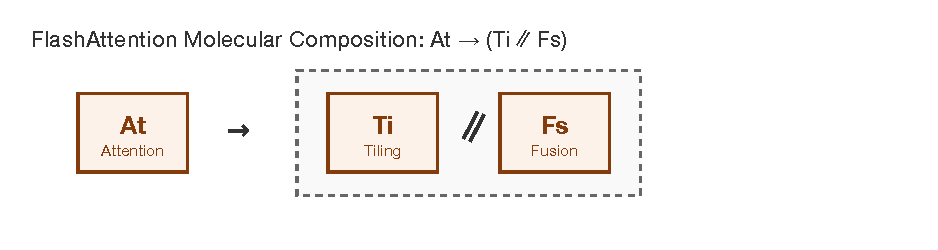
\includegraphics[width=\columnwidth]{figures/molecular_ml.pdf}
    \caption{\textbf{FlashAttention compound.} The algorithmic Attention (\texttt{At}) primitive bonds to runtime Tiling (\texttt{Ti}) and Kernel Fusion (\texttt{Fs}), keeping intermediates in SRAM rather than HBM.}
    \label{fig:flashattn}
\end{figure}

% ============================================================================
\section{Validation: Four Walkthroughs Across the Constraint Space}
\label{sec:validation}

A single walkthrough cannot validate a generative framework. The FlashAttention derivation in \Cref{sec:walkthrough} showed the four filters resolving a single-device capacity violation, but a reviewer reasonably wants to know whether the same machinery also handles other constraint types (fragmentation, multi-device capacity), other hardware contexts (NVLink vs.\ InfiniBand, datacenter vs.\ edge), and---crucially---whether it can rule things \emph{out} as well as in. This section answers those questions through four additional walkthroughs, chosen so that each one stresses a different facet of the framework.

\paragraph{What each walkthrough is designed to test.} The four are not redundant: each one introduces a constraint type or hardware context that the previous walkthroughs did not exercise.

\begin{itemize}[nosep, leftmargin=*]
\item \textbf{\Cref{sec:walkthrough} (FlashAttention)} establishes the basic four-stage pattern on a single-device, single-constraint, single-intervention case. It is the simplest possible test: one constraint binds, one filter chain prunes the candidates, one intervention resolves it.
\item \textbf{\S\ref{sec:zero-3}} (ZeRO-3) tests the heuristic on a \emph{multi-device capacity} constraint and demonstrates a \emph{cascade}: resolving one constraint introduces another (capacity $\to$ bandwidth), which the framework handles by composing two interventions instead of one.
\item \textbf{\S\ref{sec:paged-attention}} (PagedAttention) tests a \emph{fragmentation} constraint---a non-capacity, non-bandwidth bottleneck---and shows the heuristic selecting Virtualization where simpler techniques (Caching, Tiling) would fail their preconditions.
\item \textbf{\S\ref{sec:tensor-parallel}} (Megatron-LM tensor parallelism) tests \emph{the same constraint type} as ZeRO-3 (multi-device capacity) but with \emph{different hardware context} (intra-node NVLink instead of cross-node InfiniBand), and shows the framework selecting a \emph{different} intervention. This is the strongest evidence that the heuristic is sensitive to hardware context, not just constraint type.
\item \textbf{\Cref{sec:edge-analysis}} (million-token edge inference) tests the framework on an \emph{unsolved} problem with \emph{three simultaneous binding constraints}, and includes a dead-end analysis showing the heuristic pruning two plausible-but-wrong candidates before producing a viable cascade.
\end{itemize}

The five walkthroughs together cover four constraint types (single-device capacity, multi-device capacity, fragmentation, simultaneous), three hardware contexts (NVLink intra-node, InfiniBand cross-node, edge SoC), and both the affirmative case (this is the right intervention) and the rejection case (these candidates fail their preconditions). We follow the same four-stage pattern in each---na\"ive molecule, binding constraint, constraint-driven search, optimized molecule---so that the structure remains comparable, but the prose between stages is calibrated to highlight what is new.

\subsection{ZeRO-3: Distributed Training Under Memory Constraints}
\label{sec:zero-3}

\subsubsection{Stage 1: The Na\"ive Molecule}

Na\"ive data-parallel training replicates the full model state on every device:
\begin{equation*}
M_{\text{naive-dp}} = [Pm \otimes Os \otimes Ad]_{\langle \cdot \rangle_{\text{Hb}}}^{\text{per device}} \rightarrow Vu \rightarrow Sy
\end{equation*}

\subsubsection{Stage 2: The Binding Constraint}

\begin{napkinmath}{ZeRO-3 memory budget}
For a 70B parameter model in mixed-precision training (Rule~1):
\begin{align*}
\text{mem}(Pm) &= 70\text{B} \times 2\;\text{bytes (FP16)} = \cvalint{\LLaMAWeightsGB}\;\text{GB} \\
\text{mem}(Ad) &= 70\text{B} \times 2\;\text{bytes (FP16)} = \cvalint{\LLaMAWeightsGB}\;\text{GB} \\
\text{mem}(Os) &= 70\text{B} \times 12\;\text{bytes}^{\dagger} = 840\;\text{GB}
\end{align*}

\footnotesize{${}^{\dagger}$Adam: FP32 copy (4B) + first moment (4B) + second moment (4B) = 12 bytes/param.}

\normalsize
\textbf{Total per-device:} $\cvalint{\LLaMAWeightsGB} + \cvalint{\LLaMAWeightsGB} + 840 = \cvalint{\ZeROMemGB}$\,GB.

\textbf{H100 HBM:} \cvalint{\HhHBMGB}\,GB. Exceeded by $\cvalint{\ZeROMinDevices}\times$.
\end{napkinmath}

\subsubsection{Stage 3: Constraint Resolution}

\paragraph{Filter 1 (Layer).} HBM capacity, Hardware layer. Runtime candidates: $\{$Ti, Fs, Pf, Cc, Sc, Vr$\}$. Optimization-layer: $\{$Qz, Fc, Sy$\}$.

\paragraph{Filter 2 (Role).} Capacity $\Rightarrow$ Represent or Communicate. $\{$Ti, Vr, Cc, Qz, Fc, Sy$\}$.

\paragraph{Filter 3 (Constraint type).} Capacity exceeded, multi-device context: $\{$Sy, Vr, Qz, Fc$\}$.

\paragraph{Filter 4 (Hardware context).} Exact FP16 gradients required $\Rightarrow$ eliminate Qz. No general low-rank structure $\Rightarrow$ eliminate Fc. Vr addresses fragmentation, not aggregate capacity $\Rightarrow$ eliminate Vr.

\paragraph{Result.} \fbox{\texttt{Sync/Collective (Sy)}}---sharding---with \texttt{Prefetching (Pf)} as companion. This corresponds to rewrite Rule~3 in \Cref{tab:rewrite-rules}.

\subsubsection{Stage 4: The Optimized Molecule}

\begin{equation*}
M_{\text{ZeRO-3}} = \left[\underbrace{Pf \xrightarrow{bw} Sy}_{\text{gather } \ell{+}1} \;\parallel\; \underbrace{Vu}_{\text{compute } \ell}\right]^{L}
\end{equation*}
with residency $\langle Pm/N \otimes Os/N \otimes Ad/N \rangle_{\text{Hb}}$.

\begin{napkinmath}{ZeRO-3 compute vs.\ communication}
With $N = 16$ GPUs and a 70B model ($L = 80$ layers, ${\sim}$0.875B params/layer):

\textbf{All-gather time per layer (NVLink, 8 GPUs/node):}
\[
T_{\text{gather}}^{\text{NVL}} = \frac{0.875\text{B} \times 2\;\text{bytes}}{\cvalint{\NVLinkBWGBs}\;\text{GB/s}} = \frac{1.75\;\text{GB}}{900\;\text{GB/s}} \approx 1.9\;\text{ms}
\]

\textbf{All-gather time per layer (InfiniBand, cross-node):}
\[
T_{\text{gather}}^{\text{IB}} = \frac{1.75\;\text{GB}}{\cvalint{\IBBWGBs}\;\text{GB/s}} \approx 35\;\text{ms}
\]

\textbf{Compute time per layer} (forward + backward, batch size 4, seq len 4096):
\[
T_{\text{compute}} = \frac{6 \times 0.875 \times 10^9 \times 4 \times 4096}{\cvalint{\HhPeakTFLOPS} \times 10^{12}} \approx 87\;\text{ms}
\]

\textbf{Verdict:} NVLink: $T_{\text{compute}} \gg T_{\text{gather}}^{\text{NVL}}$---prefetching fully hides communication. InfiniBand: margin is thin ($2.5\times$). At smaller models, InfiniBand becomes the bottleneck---which is why ZeRO-3 uses gradient accumulation to increase $T_{\text{compute}}$.
\end{napkinmath}

Per-device memory drops to $\cvalint{\ZeROMemGB} / 16 = 70$\,GB, fitting comfortably in the \cvalint{\HhHBMGB}\,GB H100 HBM. But the optimized molecule reveals something the FlashAttention walkthrough did not: a \emph{constraint cascade}. Sharding the model state ($Sy$) resolved the capacity constraint ($\mid_{\text{cap}}$) but introduced a new bandwidth constraint ($\mid_{\text{bw}}$)---every layer now needs to all-gather its weights from peer devices before it can compute. The framework's response was to compose two interventions rather than one: $Sy$ for the capacity violation, $Pf$ (prefetching) to hide the new communication latency behind the previous layer's compute. The constraint operator generalizes naturally: $M \mid_{\text{cap}} \to M' \mid_{\text{bw}} \to M''$, with each violation triggering its own filter pass. This cascade pattern recurs in every multi-device walkthrough.

\paragraph{What this walkthrough demonstrates.} The four filters select \emph{Sync/Collective (Sy)} over the alternatives (Quantization, Factorization, Virtualization) by elimination---the rejected candidates fail their preconditions, not because of a beauty contest. And the resulting molecule is not a single intervention but a coordinated pair, derived from the cascade structure of the constraint chain. This is the first piece of evidence that the heuristic produces \emph{compositional} answers, not just point fixes.

\subsection{PagedAttention: Serving Under Memory Fragmentation}
\label{sec:paged-attention}

ZeRO-3 demonstrated the framework on a capacity constraint. PagedAttention demonstrates it on something the table's earlier examples do not exercise: a \emph{fragmentation} constraint. Fragmentation is qualitatively different from capacity. The aggregate memory used is small, but the layout makes that memory unusable---the system has space but cannot allocate it contiguously. This forces the framework to select interventions from a different region of the constraint-intervention matrix (\Cref{tab:resolution-matrix}), and the four filters must distinguish between superficially similar candidates (Caching, Tiling, Virtualization) that have very different preconditions.

\subsubsection{Stage 1: The Na\"ive Molecule}

During autoregressive generation, each request maintains a contiguous KV-cache in HBM:
\begin{equation*}
M_{\text{naive-serve}} = Hs_{\langle \text{Hb},\, \text{contig} \rangle} \rightarrow At \rightarrow Dd \;\bigm|_{\text{alloc}}
\end{equation*}
with the allocation constraint $\text{alloc} = \text{contiguous}$.

\subsubsection{Stage 2: The Binding Constraint}

For a 70B model with 80 layers and 64 KV-heads of dimension 128, each token's KV-cache entry consumes $2 \times 80 \times 64 \times 128 \times 2 = 2.6$\,MB. A request with maximum context 8,192 tokens requires ${\sim}21$\,GB of \emph{contiguous} HBM---but may only generate 500 tokens. Fragmentation:
\begin{equation*}
\text{Fg} = \frac{\text{allocated} - \text{used}}{\text{allocated}} = \frac{21 - 1.3}{21} \approx 94\%
\end{equation*}

With 4 concurrent requests, 84\,GB is allocated (exceeding \cvalint{\HhHBMGB}\,GB HBM), though only 5.2\,GB is used.

\subsubsection{Stage 3: Constraint Resolution}

\paragraph{Filters 1--3.} Fragmentation constraint $\Rightarrow$ Runtime layer, Represent/Control roles: $\{$Vr, Cc, Sc$\}$.

\paragraph{Filter 4.} KV-cache is \emph{variable-length} and \emph{dynamically growing}: Vr's preconditions are satisfied.

\paragraph{Result.} \fbox{\texttt{Virtualization (Vr)}}: map logical blocks to non-contiguous physical pages. This corresponds to rewrite Rule~4 in \Cref{tab:rewrite-rules}.

\subsubsection{Stage 4: The Optimized Molecule}

\begin{equation*}
M_{\text{paged}} = Hs \rightarrow Vr \rightarrow Cc_{\langle \text{pages} \rangle_{\text{Hb}}} \rightarrow Sc
\end{equation*}

Fragmentation drops from $>90\%$ to $<4\%$ \citep{kwon2023vllm}. Virtualization decouples logical structure from physical layout---the same principle that motivated virtual memory in operating systems half a century ago, now applied to GPU HBM half a century later. The structural similarity is not coincidence: both arise when a fixed physical resource must serve dynamically-sized, dynamically-arriving requests. The framework surfaces this connection naturally because Vr's metadata---preconditions $=$ \{variable-length-data, dynamically-growing\}---encodes the abstract pattern, not the implementation.

\paragraph{What this walkthrough demonstrates.} Filters can distinguish between candidates that look interchangeable on the surface. Caching and Virtualization both ``manage memory,'' but their preconditions differ sharply: Cc requires temporal reuse, Vr requires variable-length data. Without the filter machinery, students would pattern-match to whichever they had recently seen. With it, they reason from preconditions and arrive at the answer mechanically.

\subsection{Tensor Parallelism: Inference Under Single-Device Capacity}
\label{sec:tensor-parallel}

The third walkthrough is the most pointed test of the framework's claim to be sensitive to hardware context. The constraint type is identical to ZeRO-3's---multi-device capacity---but the deployment context is different: a small, NVLink-connected cluster doing inference rather than a large, InfiniBand-connected one doing training. Identical constraint, different hardware: should the framework propose a different intervention? It should, and it does. This walkthrough shows the four filters surfacing tensor parallelism (Megatron-LM) instead of ZeRO sharding, with the divergence happening entirely at Filter 4 (hardware context). If the framework were merely a constraint-to-technique lookup table, this discrimination would be impossible.

\subsubsection{Stage 1: The Na\"ive Molecule}

Inference of a 70B model on a single device:
\begin{equation*}
M_{\text{naive-infer}} = Pm_{\langle \text{Hb} \rangle} \rightarrow [Dd \rightarrow \text{Sm} \rightarrow Dd]^{L}
\end{equation*}

\subsubsection{Stage 2: The Binding Constraint}

\begin{napkinmath}{Tensor parallelism capacity constraint}
\textbf{Model weights:} 70B $\times$ 2 bytes (FP16) = \cvalint{\LLaMAWeightsGB}\,GB.

\textbf{Single H100 HBM:} \cvalint{\HhHBMGB}\,GB.

\textbf{Deficit:} $\cvalint{\LLaMAWeightsGB} / \cvalint{\HhHBMGB} = 1.75\times$ oversubscription. The model does not fit on one device, even before KV-cache and activation memory.

The constraint is \textbf{capacity (multi-device)}: weights must be distributed across devices.
\end{napkinmath}

\subsubsection{Stage 3: Constraint Resolution}

\paragraph{Filter 1 (Layer).} HBM capacity, Hardware layer. Runtime + Optimization candidates.

\paragraph{Filter 2 (Role).} Capacity $\Rightarrow$ Represent or Communicate: $\{$Sy, Vr, Qz, Fc, Ti$\}$.

\paragraph{Filter 3 (Constraint type).} Capacity exceeded, multi-device: $\{$Sy, Vr, Qz$\}$.

\paragraph{Filter 4 (Hardware context).} Inference requires exact weights (no training tolerance for quantization noise at this scale) $\Rightarrow$ Qz is a secondary option. KV-cache is not the bottleneck here $\Rightarrow$ Vr does not address weight capacity. NVLink cluster with $N = \cvalint{\TPdevices}$ GPUs available.

\paragraph{Result.} \fbox{\texttt{Sync/Collective (Sy)}}---specifically, \emph{column-parallel} weight sharding with all-reduce after each layer's forward pass. This is Megatron-LM tensor parallelism \citep{shoeybi2019megatron}, corresponding to rewrite Rule~5 in \Cref{tab:rewrite-rules}.

\subsubsection{Stage 4: The Optimized Molecule}

\begin{equation*}
M_{\text{TP}} = [(Pm/N)_{\langle \text{Hb} \rangle} \rightarrow Dd \rightarrow Sy_{\text{all-reduce}}]^{L}
\end{equation*}

\begin{napkinmath}{Tensor parallelism communication overhead}
With $N = \cvalint{\TPdevices}$ GPUs on NVLink (\cvalint{\NVLinkBWGBs}\,GB/s):

\textbf{Per-device weights:} $\cvalint{\LLaMAWeightsGB} / \cvalint{\TPdevices} = \cval{\TPweightsPerDevice}$\,GB. Fits in \cvalint{\HhHBMGB}\,GB HBM.

\textbf{All-reduce per layer.} Each transformer layer produces a hidden-state output of dimension $h = 8192$ (for a 70B model). The all-reduce volume per layer:
\[
|Y| = B \times s \times h \times 2\;\text{bytes}
\]
For $B = 1$, $s = 1$ (autoregressive decode): $|Y| = 16$\,KB.

\textbf{All-reduce latency} (ring, $\gamma = 2(N{-}1)/N = 1.75$):
\[
T_{\text{AR}} = \gamma \cdot \frac{16\;\text{KB}}{\cvalint{\NVLinkBWGBs}\;\text{GB/s}} + 1\;\mu\text{s} \approx 1.03\;\mu\text{s}
\]

\textbf{Compute time per layer} (single token):
\[
T_{\text{compute}} = \frac{2 \times (70/80) \times 10^9}{\cvalint{\TPdevices} \times \cvalint{\HhPeakTFLOPS} \times 10^{12}} \approx 0.22\;\text{ms}
\]

\textbf{Ratio:} $T_{\text{compute}} / T_{\text{AR}} \approx 214\times$. Communication overhead is negligible on NVLink. On InfiniBand (50\,GB/s, 5\,$\mu$s latency), the ratio drops to ${\sim}12\times$---still viable, but NVLink's $\cvalint{\NVLinkIBgap}\times$ bandwidth advantage explains why tensor parallelism is preferred \emph{within} a node.
\end{napkinmath}

The framework derives not only the \emph{intervention} (sharding) but also the \emph{topology constraint} (NVLink-connected devices) from the bandwidth analysis itself. Tensor parallelism across InfiniBand is possible but inefficient; the napkin math reveals why practitioners keep TP within an NVLink domain and use pipeline or data parallelism across nodes \citep{narayanan2021efficient}.

\paragraph{What this walkthrough demonstrates.} The same constraint type (multi-device capacity) produced \emph{different} interventions in ZeRO-3 (Sy + Pf, optimized for InfiniBand) and Megatron-LM (Sy + AllReduce, optimized for NVLink). The divergence happened at Filter 4, where hardware context discriminated between the candidates that survived Filters 1--3. This is the framework's strongest claim to be more than a labeling system: identical constraints under different hardware produce different molecules, and the discrimination is mechanical, not heuristic. A taxonomy cannot do this.

\paragraph{Three walkthroughs in, what we have shown.} ZeRO-3 demonstrated cascading constraints. PagedAttention demonstrated precondition-based discrimination among similar candidates. Tensor parallelism demonstrated hardware-context sensitivity. The fourth walkthrough now turns the framework against an \emph{open} problem and asks the question reviewers most often ask of derivation frameworks: does it work when there is no published answer to derive toward?

\subsection{Forward-Looking Analysis: Million-Token Context on Edge}
\label{sec:edge-analysis}

The strongest test is whether the framework structures reasoning about \emph{unsolved} problems. We apply it to serving a model with \EdgeCtxTokens{}-token context on a unified-memory edge device (Apple M4 Pro: \cvalint{\EdgeRAMGB}\,GB unified RAM, \cvalint{\EdgeBWGBs}\,GB/s bandwidth, \cvalint{\EdgeTFLOPS}\,TOPS).

\begin{napkinmath}{Million-token KV-cache on edge}
For a 7B model (32 layers, 32 KV-heads, head dim 128):

\textbf{KV per token:} $2 \times 32 \times 32 \times 128 \times 2 = \cval{\EdgeKVPerTokenMB}$\,MB.

\textbf{KV at \EdgeCtxTokens{} tokens:}
\[
\cval{\EdgeKVPerTokenMB}\;\text{MB} \times \EdgeCtxTokensRaw{} = \EdgeKVTotalGB{}\;\text{GB}
\]

\textbf{Exceeds \cvalint{\EdgeRAMGB}\,GB unified memory by ${\sim}13\times$.}

Three constraints bind simultaneously:
\begin{enumerate}[nosep]
\item \textbf{Capacity:} KV-cache exceeds memory by $13\times$.
\item \textbf{Bandwidth:} \cvalint{\EdgeBWGBs}\,GB/s is $12\times$ slower than H100 HBM; streaming full KV per token takes ${\sim}1.7$\,s.
\item \textbf{Compute:} $O(n^2)$ attention at this scale on \cvalint{\EdgeTFLOPS}\,TOPS is catastrophic.
\end{enumerate}
\end{napkinmath}

\paragraph{Constraint-driven search: showing the dead ends.} The value of the heuristic is not that it lists the right techniques---any survey can do that. The value is that it \emph{prunes wrong paths with napkin math before the engineer wastes time implementing them}. We show the search tree with its dead ends.

\begin{errorcase}{Dead end 1: Ring Attention on M4 Pro}
\textbf{Candidate.} The heuristic's capacity filter surfaces Ring Attention \citep{liu2023ring} as an intervention for the $O(n^2)$ memory constraint: distribute the KV-cache across devices via a ring of attention tiles.

\textbf{Why it fails.} Ring Attention requires multiple devices with high-bandwidth interconnect. The M4 Pro is a \emph{single SoC}. There is no ring. Even if we treated CPU and GPU as separate ``devices,'' the M4 Pro's unified memory architecture means there is no bandwidth gain from partitioning---both access the same \cvalint{\EdgeBWGBs}\,GB/s memory bus.

\textbf{Filter 4 (Hardware context):} $\text{RingAt}.\text{preconditions} = \{$multi-device, point-to-point interconnect$\}$. $\{$multi-device$\} \not\subseteq \mathcal{P}_{\text{M4 Pro}}$. \emph{Eliminated.}

\textbf{Napkin math confirms:} Even hypothetically, ring communication across Thunderbolt ($\sim$5\,GB/s) would add $\EdgeKVTotalGB / 5 \approx 95$\,s per token. Catastrophic. \emph{Pruned.}
\end{errorcase}

\begin{errorcase}{Dead end 2: Tiling alone (FlashAttention-style)}
\textbf{Candidate.} Tiling resolved the attention memory bottleneck on H100 (\Cref{sec:walkthrough}). Can it work here?

\textbf{Why it is insufficient.} Tiling reduces \emph{intermediate} memory ($S = QK^T$) from $O(n^2)$ to $O(B^2)$. But the KV-cache itself---$\EdgeKVTotalGB$\,GB---is not an intermediate; it is \emph{state} that must persist across tokens. Tiling does not reduce persistent state.

\textbf{Napkin math:} After tiling, intermediate memory drops to $\sim$128\,KB per tile. But KV-cache remains at $\EdgeKVTotalGB$\,GB. The capacity constraint is still violated by $13\times$. Tiling is \emph{necessary but not sufficient}---it must be combined with KV compression.
\end{errorcase}

\paragraph{The viable cascade.} After pruning Ring Attention and standalone Tiling, the heuristic produces a cascade of interventions, each resolving one constraint while possibly introducing another:

\begin{itemize}[nosep]
\item \textbf{Capacity (first pass):} Qz (quantize KV to INT4: $4\times$ reduction $\Rightarrow$ 119\,GB). Still exceeds \cvalint{\EdgeRAMGB}\,GB.
\item \textbf{Capacity (second pass):} Fc (low-rank KV approximation: $2\times$ $\Rightarrow$ 60\,GB). Still $1.7\times$ over.
\item \textbf{Capacity (third pass):} Vr (disk-backed paging: active working set $\sim$4\,GB fits in RAM).
\item \textbf{Bandwidth:} Pf (prefetch next context window from SSD during compute).
\item \textbf{Compute:} The $O(n^2)$ cost at this scale requires a sub-quadratic attention mechanism---an Algorithm-layer intervention. Candidates: sparse attention ($O(n \sqrt{n})$), linear attention ($O(n)$).
\end{itemize}

\paragraph{The final molecule.}

\begin{equation*}
M_{\text{edge}} = [Ti \rightarrow (Dd_{\text{sparse}} \rightarrow \text{Sm})_{\langle\text{Sr}\rangle}]^{n/B} \rightarrow Fs
\end{equation*}
with KV residency:
\begin{equation*}
Hs \rightarrow Qz_{\text{INT4}} \rightarrow Fc \rightarrow Vr_{\langle\text{SSD} \to \text{RAM}\rangle} \rightarrow Pf
\end{equation*}

\begin{napkinmath}{Closed-loop edge verification}
\textbf{After INT4 quantization + $2\times$ factorization:}
\[
\text{KV}_{\text{compressed}} = \frac{\EdgeKVTotalGB{}}{4 \times 2} = 60\;\text{GB}
\]

Still $1.7\times$ over \cvalint{\EdgeRAMGB}\,GB. Virtualization (Vr) pages the overflow to SSD; active working set per decode step: ${\sim}$4\,GB (recent context window).

\textbf{Bandwidth after compression:} Streaming 4\,GB working set:
\[
T_{\text{stream}} = \frac{4\;\text{GB}}{\cvalint{\EdgeBWGBs}\;\text{GB/s}} \approx 15\;\text{ms/token}
\]

\textbf{With sub-quadratic attention} ($O(n\sqrt{n})$, $\sqrt{10^6} = 1000$ effective window):
\[
T_{\text{compute}} = \frac{2 \times 7 \times 10^9 \times 1000}{\cvalint{\EdgeTFLOPS} \times 10^{12}} \approx 0.26\;\text{ms}
\]

\textbf{Bottleneck:} Memory bandwidth at 15\,ms/token (${\sim}$67 tok/s). Acceptable for edge. The ridge point analysis confirms the system is bandwidth-bound ($I \approx 3.5$\,FLOP/byte vs.\ $I^* \approx 194$\,FLOP/byte for M4 Pro).

\textbf{Structural prediction:} Any viable million-token edge solution will contain \{Qz, Fc, Vr, Pf, sub-quadratic At\} or their functional equivalents. A paper that achieves this without one of these components must have found a qualitatively different approach.

\textbf{What the dead ends prove:} The framework did not merely list the answer---it pruned Ring Attention (wrong hardware context) and standalone Tiling (wrong constraint scope) \emph{before} arriving at the viable cascade. Showing the search tree's pruned branches is what distinguishes a generative framework from a retrospective taxonomy.
\end{napkinmath}

\paragraph{What the edge walkthrough demonstrates.} On an unsolved problem with three simultaneous binding constraints, the framework produced a structurally specified molecule, predicted the components any viable solution must contain, and showed its work---including the wrong paths it considered and rejected. The molecule is not a recipe; it is a class of solutions, and any specific paper that ships a million-token edge model will be an instance of this class. This is what generative means: not ``the framework outputs the answer'' but ``the framework constrains the answer space tightly enough that the answer becomes structurally inevitable.''

\paragraph{Synthesis: what the five walkthroughs collectively show.} Across FlashAttention, ZeRO-3, PagedAttention, Megatron-LM, and the edge analysis, the same four-filter procedure operated on the same 90-element table and produced five qualitatively different molecules. The differences trace cleanly to the inputs: different constraint type (capacity vs.\ fragmentation), different scope (single-device vs.\ multi-device), different hardware context (NVLink vs.\ InfiniBand vs.\ unified memory), different interaction (single intervention vs.\ cascade vs.\ simultaneous constraints). In each case, every filter step was deterministic, every elimination was justified by metadata, and every output corresponded to either a published system or---in the edge case---a structurally predicted future system. The framework does not need to know about FlashAttention to derive FlashAttention. It needs to know about Tiling, Fusion, SRAM, and the irreducibility of Attention. The published name is the consequence; the periodic-table primitives plus the constraint-driven search are the cause. This is the empirical case for the framework.

% ============================================================================
\section{Beyond the Single Node: Probabilistic Constraints}
\label{sec:probabilistic}

Deterministic constraints govern the \emph{node}. Stochastic constraints govern the \emph{fleet}. This distinction is the central engineering challenge of hyperscale ML. A system that works on 8 GPUs and fails at 1,024 has not encountered an unusual condition; it has encountered the \emph{normal operating regime} of distributed training.

\subsection{The Generalized Constraint Operator}

In \Cref{sec:composition}, we introduced the generalized constraint operator:
\begin{equation}
M \;\mid_{C,\; p > \theta} \quad \xRightarrow{\;P(C\text{ violated}) > \theta\;} \quad \text{\textsc{Search}}(M, C) = M'
\end{equation}
For deterministic constraints ($\theta = 0$), any violation triggers search---this is the regime of \Cref{sec:walkthrough,sec:validation}. For probabilistic constraints ($\theta > 0$), the trigger is a probability threshold. The Stochastic Variance element (\texttt{Sv}) measures the tail distribution that determines $P(C\text{ violated})$.

\subsection{The Straggler Problem}

\begin{errorcase}{Stragglers in distributed all-reduce}
\textbf{Scenario.} A 1,024-GPU training job runs ring all-reduce across 128 nodes. The deterministic model (Rule~4) predicts:
\begin{align*}
T_{\text{all-reduce}} &= \gamma \cdot \frac{|G|}{bw} + \alpha \\
&= \tfrac{2 \times 1023}{1024} \cdot \tfrac{26\;\text{GB}}{50\;\text{GB/s}} + 5\;\mu\text{s} \\
&\approx 1.04\;\text{s}
\end{align*}

\textbf{What actually happens.} At 1,024 GPUs, the probability that \emph{at least one} node experiences a transient slowdown per step:
\begin{align*}
P(\text{straggler}) &= 1 - (1 - p)^{128} \\
&\approx 1 - (0.99)^{128} \approx 72\%
\end{align*}

A single straggler running $3\times$ slower turns $T_{\text{all-reduce}}$ from 1.04\,s to 3.1\,s. The deterministic framework misses this because $\mid_C$ assumes deterministic bounds. Straggler effects are \emph{probabilistic}: $P(\text{violation}) > 0$ even when $\text{mean}(C)$ is satisfied.
\end{errorcase}

\subsection{Applying the Generalized Operator}

Setting $\theta = 0.5$: when $P(\text{straggler}) = 72\% > \theta$, the generalized constraint operator fires. The four-filter heuristics correctly surface Control-role interventions:

\begin{napkinmath}{Straggler mitigation cost}
\textbf{Without mitigation:} Expected per-step time:
\[
E[T] = 0.28 \times 1.04 + 0.72 \times 3.1 \approx 2.5\;\text{s}
\]

\textbf{With redundant computation (2\% overhead):} Launch backup all-reduce on alternate paths; the faster path completes. Expected time drops to about 1.1\,s---a $2.3\times$ improvement for 2\% compute overhead.

\textbf{Filter result:} Layer $\to$ Production/Runtime. Role $\to$ Control. Hardware context $\to$ multi-node with synchronization barrier. Candidates: \textbf{Sc} (topology-aware scheduling), \textbf{Or} (redundant execution, bounded staleness). This matches Google's production approach \citep{dean2013tail}.
\end{napkinmath}

\paragraph{The boundary.} The deterministic framework (\Cref{sec:walkthrough,sec:validation}) is accurate within one node and progressively less so as fleet size grows. The generalized operator formalizes \emph{where} the boundary lies ($P(\text{straggler}) > \theta$) and \emph{what replaces} the deterministic trigger. Fully integrating probabilistic constraints into the cost rules---so that \texttt{Sv} participates in the four-filter search as a first-class input---is the most important open formalization challenge.

% ============================================================================
\section{The Framework as a Teaching Tool}
\label{sec:teaching}

The previous sections built the framework as a research artifact: a design space, a search heuristic, and a cost calculus. This section reframes the same machinery as a curriculum. The argument is that the things we built for derivation---irreducibility, four filters, cost rules---turn out to be exactly the things students need to develop transferable intuition. The framework's pedagogical value is not an afterthought; it falls out of the formal structure once you stop thinking like a researcher and start thinking like an instructor at a whiteboard.

The section unfolds in three movements. First, we distill the framework into manipulable equations and a structured whiteboard protocol that students can apply by hand (\Cref{sec:iron-laws,sec:whiteboard}). Second, we work through examples that show what teaching with these tools looks like in practice---a routine sizing problem, a forward-derivation exercise, and a failure case where the filters catch a wrong answer (\Cref{sec:kv-sizing,sec:predict-paper,sec:failure-case}). Third, we present the curricular machinery: an exercise bank graded from single-node to fleet-scale, integration with two existing platforms, and preliminary deployment evidence from a Harvard course (\Cref{sec:exercises,sec:curriculum,sec:deployment}). The thread connecting all three is that every step of the framework---a constraint, a filter, a primitive---is an item a student can name, manipulate, and defend at a whiteboard. The pedagogy is not added on top; it is the same machinery rotated toward learning.

\subsection{The Iron Laws of ML Systems}
\label{sec:iron-laws}

Just as Patterson and Hennessy's Iron Law of processor performance ($\text{Time} = \text{IC} \times \text{CPI} \times T_{\text{clk}}$) gives students a manipulable equation for reasoning about CPU design, the framework yields three canonical equations that decompose ML system performance into physically meaningful terms. Each Iron Law collapses the cost rules of \Cref{sec:cost-model} into a single inequality or formula that fits on a whiteboard, and each one can be manipulated symbolically: students can substitute hardware specifications, solve for unknowns, and predict which constraint binds first as parameters scale.

\paragraph{Iron Law 1: Memory Capacity.} A model fits on $N$ devices if and only if:
\begin{align}
\label{eq:iron-capacity}
&\underbrace{P \cdot b_w}_{\text{weights}} \;+\; \underbrace{P \cdot b_o}_{\text{optimizer}} \;+\; \underbrace{B \cdot s \cdot h \cdot L \cdot b_a}_{\text{activations}} \notag \\
&\quad +\; \underbrace{2 \cdot L \cdot n_{\text{kv}} \cdot d \cdot s \cdot b_k}_{\text{KV-cache}} \;\leq\; N \cdot C_{\text{HBM}}
\end{align}
where $P$ is parameters, $b_w$ is bytes per weight, $b_o$ is bytes per optimizer state (12 for Adam), $B$ is batch size, $s$ is sequence length, $h$ is hidden dimension, $L$ is layers, $n_{\text{kv}}$ is KV-heads, $d$ is head dimension, $b_a$ and $b_k$ are bytes per activation and KV entry, and $C_{\text{HBM}}$ is per-device HBM capacity. Each term maps to a Represent-role element; each $\leq$ is a constraint operator $\mid_{\text{CAP}}$.

\paragraph{Iron Law 2: Throughput Bound.} Per-token throughput is:
\begin{equation}
\label{eq:iron-throughput}
\text{Tokens/s} \;=\; \bigl[\, T_{\max} + \delta_{\text{bubble}} \,\bigr]^{-1},
\end{equation}
where $T_{\max}$ is the binding-constraint time:
\begin{equation}
\label{eq:iron-throughput-tmax}
T_{\max} = \max\!\left(\underbrace{\tfrac{2P}{N \pi}}_{\text{compute}},\;\; \underbrace{\tfrac{P \cdot b_w}{N \beta}}_{\text{bandwidth}},\;\; \underbrace{\tfrac{\gamma |G|}{bw_{\text{net}}}}_{\text{comm}}\right).
\end{equation}
where $\pi$ is per-device peak FLOP/s, $\beta$ is memory bandwidth, $bw_{\text{net}}$ is network bandwidth, $|G|$ is gradient size, $\gamma$ is the collective scaling factor, and $\delta_{\text{bubble}}$ is the pipeline bubble overhead from \Cref{eq:bubble}. The $\max$ identifies the binding constraint; the additive $\delta_{\text{bubble}}$ captures the concurrency overhead that simpler models ignore.

\paragraph{Iron Law 3: Serving Efficiency.} For inference, the arithmetic intensity is:
\begin{equation}
\label{eq:iron-serving}
I = \frac{2P \cdot B}{P \cdot b_w} = \frac{2B}{b_w} \;\text{FLOP/byte}
\end{equation}
At batch size $B = 1$ with FP16 weights ($b_w = 2$): $I = 1$ FLOP/byte. The ridge point on H100 is 295. The system is $295\times$ below peak---and the only lever is $B$. This is why continuous batching exists: it is not a software optimization but a \emph{physical necessity} for efficient hardware utilization.

\paragraph{Why three laws are enough.} Capacity, throughput, and serving efficiency are not arbitrary choices. Capacity is the constraint that fails first (the model must fit before anything else matters); throughput is the constraint that determines training cost (which is what funds the next model); and serving efficiency is the constraint that determines inference economics (which is what funds the next deployment). Every other ML systems equation a student is likely to encounter---scaling laws, FLOP-utilization estimates, latency budgets---is a special case of one of these three. Treating them as the first equations on the whiteboard means students learn a small, complete vocabulary that generalizes, rather than a sprawling collection of named formulas.

\subsection{The Whiteboard Protocol}
\label{sec:whiteboard}

The Iron Laws give students the equations; the whiteboard protocol gives them the procedure. In classroom and interview settings, the four-stage walkthrough used throughout \Cref{sec:walkthrough,sec:validation} becomes a four-step protocol that an instructor can use to lead a discussion or that a candidate can use to structure an answer:

\begin{enumerate}[nosep, leftmargin=*]
\item \textbf{Write the na\"ive molecule.} Decompose the system into irreducible primitives.

\item \textbf{Annotate with hardware specs and compute costs.} Attach memory residency, apply Rules 1--4.

\item \textbf{Run the four filters.} Write the candidate set and cross out elements as each filter prunes. This makes reasoning visible and debuggable.

\item \textbf{Verify the optimized molecule.} Re-evaluate Rules 1--4. Confirm the constraint is resolved. Check for cascading constraints.
\end{enumerate}

The protocol's power lies in Step~3: when a student crosses out ``Caching (Cc)'' because the access pattern has no temporal reuse, they are learning a transferable principle about memory hierarchies---not memorizing a FlashAttention-specific fact. The crossing-out is observable: an instructor can see exactly which filter each student misapplies, and the student can see exactly where their reasoning diverged from the correct chain. This is the diagnostic value the framework adds to existing instruction.

The next three subsections show the protocol in action across three increasingly demanding settings: a routine sizing problem (\Cref{sec:kv-sizing}), where the protocol replaces ad-hoc arithmetic; a forward-derivation exercise (\Cref{sec:predict-paper}), where the protocol predicts a published system before the student sees its name; and a failure case (\Cref{sec:failure-case}), where the protocol catches an intuitive but wrong intervention. Together they show what teaching with the framework looks like.

\subsection{Worked Example: KV-Cache Sizing}
\label{sec:kv-sizing}

\paragraph{Problem.} ``You are serving a 7B model (32 layers, 32 KV-heads, head dim 128) on a single GPU with 24\,GB VRAM. Weights consume 14\,GB in FP16. How many concurrent requests at context length 4,096 can you serve?''

\begin{napkinmath}{KV-cache sizing}
\textbf{Step 1: Na\"ive molecule.}
\[
M = [Hs_{\text{contig}} \otimes Pm]_{\langle \cdot \rangle_{\text{Hb}}} \rightarrow At^L
\]

\textbf{Step 2: Hardware annotation.}
\begin{align*}
\text{Available VRAM} &= 24 - 14 = 10\;\text{GB} \\
\text{KV per token} &= 2 \times 32 \times 32 \times 128 \times 2 = 0.5\;\text{MB} \\
\text{KV per request} &= 0.5 \times 4{,}096 = 2{,}048\;\text{MB} \approx 2\;\text{GB} \\
\text{Max concurrent} &= \lfloor 10 / 2 \rfloor = \mathbf{5}
\end{align*}

\textbf{Step 3: Fragmentation.} With contiguous allocation and variable-length requests (some use 512 of 4,096 tokens): $\text{Fg} \approx 87\%$. Effective concurrency: \textbf{1--2 requests}.

\textbf{Four filters:} Layer $\to$ Runtime. Role $\to$ Represent/Control. Constraint $\to$ Fragmentation. Hardware $\to$ single GPU, variable-length state.

\textbf{Result:} \textbf{Vr} + \textbf{Cc}. With paged allocation, fragmentation $<4\%$:
\[
\text{Concurrent requests} = \left\lfloor \frac{10{,}240\;\text{MB}}{0.5 \times 512} \right\rfloor = \mathbf{40}
\]

An $8\times$ improvement. \textbf{Cascade check:} 40 requests raises compute demand $\Rightarrow$ continuous batching needed.
\end{napkinmath}

The KV-cache exercise is routine in its arithmetic but instructive in its structure. A student who has never seen PagedAttention by name still arrives at it---and at the cascade that follows---in five whiteboard steps. The exercise is also the first place where the student experiences the cascade pattern directly: resolving fragmentation immediately reveals a downstream compute constraint, exactly as the multi-device walkthroughs demonstrated. The lesson is structural: ``one fix is rarely the whole story.''

\subsection{The ``Predict the Paper'' Exercise}
\label{sec:predict-paper}

The KV-cache example tested the framework as a sizing tool. The next exercise tests it as a \emph{derivation} tool---which is the more demanding claim, because it asks students to produce a system that they have not yet seen and then verify their answer against the published literature. We call this exercise ``Predict the Paper,'' and it is the strongest pedagogical demonstration of the framework's generative claim. Given only a constraint, a hardware specification, and the four filters, students should be able to derive the architecture of a published system before the instructor reveals its name.

\paragraph{Setup.} ``Autoregressive decoding of a 70B model on a single H100: 12 tokens/s, of which 80\,ms is memory-bandwidth-bound (streaming 140\,GB weights at \cval{\HhBWTBs}\,TB/s). GPU compute is 96\% idle. Design a system achieving 100+ tokens/s.''

\begin{napkinmath}{Predict the paper: batched decoding}
\textbf{Root cause:} Arithmetic intensity at $B = 1$:
\[
I = \frac{2 \times 70 \times 10^9}{140 \times 10^9} = 1\;\text{FLOP/byte}
\]

Ridge point = 295. The kernel is $295\times$ below---massively memory-bound.

\textbf{Roofline insight:} Batching $B$ requests amortizes weight reads:
\[
I_{\text{batched}} = B \;\text{FLOP/byte}
\]

At $B = 295$, the workload reaches the ridge point.

\textbf{Filter result:} Utilization $\Rightarrow$ Sc (iteration-level scheduler). Companion: Vr (PagedAttention for managing concurrent KV-caches).
\end{napkinmath}

The instructor reveals: this is Orca/vLLM \citep{yu2022orca,kwon2023vllm}. Students experience the critical insight: they \emph{derived} a published system from constraints, without knowing its name in advance. The point is not that the framework is sufficient to invent these systems---real research involves trial, error, and engineering judgment we have not formalized---but that the framework narrows the design space tightly enough that students arrive at the same general class of solution as the published authors. The intervention is no longer mysterious; it is mechanical.

A natural question follows: what happens when students propose the wrong intervention? The framework's value depends on whether it catches mistakes as crisply as it derives correct answers. The next subsection shows exactly that.

\subsection{Failure Case: When the Filters Catch an Error}
\label{sec:failure-case}

\begin{errorcase}{Student applies wrong intervention to attention bottleneck}
\textbf{Scenario.} A student proposes \textbf{Caching (Cc)} for the attention memory bottleneck: ``Cache $QK^T$ so we don't recompute it.''

\textbf{Where the filters catch it.} Filter 4: in autoregressive generation, each new token changes $Q$ and extends $K$. The entire $QK^T$ changes every step. There is \emph{no temporal reuse}. $\text{Cc}.\text{preconditions} = \{$temporal-reuse$\} \not\subseteq \mathcal{P}$.

\textbf{Cost model confirms.} Rule 1: caching the $n \times n$ intermediate \emph{adds} \AttnTotalGB{}\,GB to HBM, \emph{worsening} the constraint: $\text{mem}(M_{\text{wrong}}) > \text{mem}(M_{\text{naive}})$.

\textbf{Lesson.} Caching resolves bandwidth constraints \emph{when temporal reuse exists}. Without reuse, caching increases memory pressure. The filters formalize this; the cost model provides the quantitative check.
\end{errorcase}

This is the diagnostic property the framework adds to existing instruction. The student's mistake is not ``you got the answer wrong''; it is ``Filter 4 was misapplied because Cc's preconditions include temporal reuse, which this access pattern lacks.'' The feedback is specific, the correction is actionable, and---crucially---the principle transfers: the next time the student encounters caching as a candidate, they will check temporal reuse first.

\subsection{Classroom Exercise Bank}
\label{sec:exercises}

The previous three subsections gave one example each of routine sizing, forward derivation, and failure diagnosis. Real classrooms need more variety than that. This subsection offers six exercises chosen to span the framework's full range: from a single-constraint compression problem on a consumer GPU (Exercise~1) to a fleet-scale probabilistic synchronization problem on 10,000 GPUs (Exercise~5), and culminating in a composition exercise that asks students to assemble all four parallelism strategies into a coherent molecule for a 1-trillion-parameter model (Exercise~6). Each exercise is graded along two axes: the constraint type it stresses, and the filter step that does the most discriminative work. The exercises are not parallel restatements of the same idea; they are designed to be assigned in sequence so that each one introduces a new dimension of the framework while reusing the machinery established by the previous one.

\begin{exercise}{Quantization Trade-Off Analysis}
A 13B model in FP16 (26\,GB weights) on a 24\,GB consumer GPU. Quantizing to INT4 reduces weights to 6.5\,GB but introduces 0.3\% perplexity degradation.

\textbf{Tasks:}
\begin{enumerate}[nosep, leftmargin=*]
\item Write the na\"ive molecule. Does capacity bind?
\item Apply Qz. Verify: $6.5 < 24$\,GB.
\item Compute arithmetic intensity change: $I_{\text{FP16}} = 1$ vs.\ $I_{\text{INT4}} = 4$\,FLOP/byte. Why?
\item Solve for $B^*$ where the quantized model becomes compute-bound: $B^* \times 4 = I^*$.
\end{enumerate}

\textbf{Key insight:} Quantization resolves capacity \emph{and} improves arithmetic intensity---a rare two-for-one.
\end{exercise}

\begin{exercise}{Pipeline Parallelism Bubble}
A 4-stage pipeline with microbatch size $m$. Bubble fraction: $(p{-}1)/(p{-}1+m)$ where $p = 4$.

\textbf{Tasks:}
\begin{enumerate}[nosep, leftmargin=*]
\item Solve for minimum $m$ such that bubble $< 10\%$.
\item Apply Rule~1: how does activation memory scale with $m$?
\item Identify the cascade: resolving utilization creates a capacity constraint. What Runtime element resolves it?
\item Write the complete optimized molecular formula.
\end{enumerate}

\textbf{Key insight:} Cascades---resolving one constraint creates another---are the most common failure mode.
\end{exercise}

\begin{exercise}{Design Your Own Element}
CXL memory expanders: 64\,GB/s bandwidth, 200--400\,ns latency.

\textbf{Tasks:}
\begin{enumerate}[nosep, leftmargin=*]
\item Apply the irreducibility criterion (\Cref{eq:irreducibility}): can CXL's cost be modeled from HBM and Host DRAM, or does it need its own cost function?
\item Define its metadata: layer, role, constraint affinity, preconditions.
\item Update the constraint-intervention matrix for capacity. When is CXL preferred over sharding?
\item Write a molecular formula using CXL as a capacity-expansion tier.
\end{enumerate}

\textbf{Key insight:} The irreducibility criterion provides a principled admission mechanism.
\end{exercise}

\begin{exercise}{Cross-Framework Comparison}
FlashAttention, Ring Attention \citep{liu2023ring}, and Sequence Parallelism all resolve the $O(n^2)$ attention memory constraint with different architectures.

\textbf{Tasks:}
\begin{enumerate}[nosep, leftmargin=*]
\item For each, write the molecular formula using $\otimes$ and $\parallel$ correctly.
\item At which filter do the three diverge? (Hint: hardware context.)
\item Using Rule~5, rank by communication overhead on a 4-node NVLink cluster.
\item Which system for $n = 1{,}000{,}000$ tokens? Why does hardware context force the answer?
\end{enumerate}

\textbf{Key insight:} Same constraint, different hardware contexts $\Rightarrow$ different architectures---mechanically.
\end{exercise}

\begin{exercise}{Tail-at-Scale: Fleet Gradient Synchronization}
A 10,000-GPU training cluster runs synchronous all-reduce gradient aggregation across 1,250 nodes (8 GPUs each). Each node has a 1\% probability of a transient slowdown ($3\times$ latency) per training step. The gradient payload is 26\,GB (13B model, FP16). InfiniBand bandwidth is \cvalint{\IBBWGBs}\,GB/s per port.

\textbf{Tasks:}
\begin{enumerate}[nosep, leftmargin=*]
\item Compute the probability that \emph{at least one} node straggles per step: $P = 1 - (1 - 0.01)^{1250}$.
\item Using the deterministic cost model (Rule~5), compute the expected all-reduce time without stragglers.
\item Compute the expected per-step time \emph{with} stragglers: $E[T] = (1{-}P) \cdot T_{\text{normal}} + P \cdot T_{\text{straggler}}$.
\item Apply the generalized constraint operator: set $\theta = 0.5$. Does $P > \theta$? What interventions do the four filters surface?
\item Design a molecule using $\parallel$ (temporal concurrency) to overlap redundant all-reduce paths. What is the overhead? What is the speedup?
\item \textbf{Challenge:} At what cluster size does asynchronous gradient descent (bounded staleness) become more efficient than redundant synchronous paths? Derive the crossover point from Rule~5 and \Cref{eq:bubble}.
\end{enumerate}

\textbf{Key insight:} At fleet scale, the constraint operator must become probabilistic. The transition from $\theta = 0$ to $\theta > 0$ is not an edge case---it is the \emph{dominant operating regime} for any cluster above ${\sim}$500 GPUs.
\end{exercise}

\begin{exercise}{Periodic Table Cheat Sheet: 1T Model on 256 GPUs}
\textbf{Given:} A 1-trillion-parameter model. 256 H100 GPUs across 32 nodes (8 GPUs/node, NVLink intra-node, InfiniBand inter-node). HBM = \cvalint{\HhHBMGB}\,GB/device. Target: $\geq$15\% of peak FLOPs utilization.

\textbf{Formal bounds:}
\begin{itemize}[nosep]
\item Iron Law 1 (\Cref{eq:iron-capacity}): weights alone $= 1\text{T} \times 2 = 2{,}000$\,GB. Per-device: $2{,}000/256 = 7.8$\,GB for weights (fits).
\item Optimizer state $= 1\text{T} \times 12 = 12{,}000$\,GB. Per-device: $46.9$\,GB. Total with weights: $54.7$\,GB $<$ \cvalint{\HhHBMGB}\,GB (fits, with 25.3\,GB remaining for activations).
\item Iron Law 2 (\Cref{eq:iron-throughput}): at batch size $B$ and sequence length $s = 4096$, compute time per step $= 6 \times 10^{12} \times B \times s / (256 \times \cvalint{\HhPeakTFLOPS} \times 10^{12})$.
\end{itemize}

\textbf{Tasks:}
\begin{enumerate}[nosep, leftmargin=*]
\item Construct a valid molecule that distributes weights, optimizer, and gradients across 256 devices. Which sharding strategy (ZeRO-1, ZeRO-2, ZeRO-3) is needed? Justify with Iron Law 1.
\item The NVLink domain is 8 GPUs. Does tensor parallelism span 8 or 32 devices? Use Rule~5 to compare NVLink vs.\ InfiniBand all-reduce latency.
\item Compute the pipeline bubble for $p = 4$ stages. What microbatch count $m$ achieves $\delta_{\text{bubble}} < 0.15 \cdot T_{\text{total}}$?
\item Write the complete molecular formula: $M = \text{TP}_8 \parallel \text{PP}_4 \parallel \text{DP}_8$ with explicit $\otimes$ for memory adjacency and $\parallel$ for temporal overlap.
\item Verify: does the molecule stay within 15\% of peak FLOPs? Show the Roofline position.
\end{enumerate}

\textbf{Key insight:} This exercise forces students to \emph{compose} all four parallelism strategies (data, tensor, pipeline, ZeRO) into a single coherent molecule, using the Iron Laws as formal bounds. The answer is not unique---multiple valid molecules exist---but all must satisfy the same capacity and throughput constraints.
\end{exercise}

The exercises share a common structure: each names a system, a constraint, and a hardware context, then asks the student to apply the four-filter procedure and arrive at an intervention that they justify with napkin math. This is not coincidence; it is the framework's pedagogy in concentrated form. By the time a student has worked through all six, they have applied every cost rule, encountered every constraint type, exercised the cascade pattern multiple times, and made the transition from deterministic to probabilistic reasoning. The exercises exist to give students reps with the same procedure across different problem instances, the way a Hennessy and Patterson chapter ends with a dozen variations on the same processor-pipeline analysis.

\subsection{Integration with Existing Platforms}
\label{sec:curriculum}

The framework does not have to live in a vacuum. Two existing platforms in the same ecosystem already consume its outputs: StaffML \citep{reddi2026staffml}, an interview framework that uses the constraint-driven heuristics as an assessment rubric, and MLSysIM \citep{reddi2026mlsysim}, a system simulator that grounds the framework's symbolic cost estimates in concrete numbers. The Periodic Table provides StaffML's vocabulary (what to test); StaffML provides the scaffolding (how to test it). MLSysIM provides the quantitative backend: a student who has reached an answer on the whiteboard can carry the same molecular formula into the simulator and check whether the predicted bottleneck actually appears under cycle-accurate execution. The three artifacts---table, interview rubric, simulator---are designed to compose, not to compete. A complete course could use all three: the table for vocabulary, StaffML for assessment, MLSysIM for verification.

For university courses specifically, the table's row structure maps cleanly onto a typical 13-week semester. Each week covers one or two rows. A student who learned Tiling in the Runtime week immediately recognizes when Tiling applies to a new constraint in the Serving week---the row provides the vocabulary, and the column provides the role-based reasoning that lets the same primitive solve different constraints in different contexts.

\subsection{Preliminary Deployment Experience}
\label{sec:deployment}

Talking about pedagogy in the abstract is easy; this subsection reports the qualitative experience of actually teaching with the framework. The intent is not to claim that the framework has been validated empirically---the controlled study we describe at the end of this subsection has not yet run---but to share the three observations that have shaped how we revise the framework between iterations.

The framework has been deployed in Harvard's CS249r (Machine Learning Systems) course across three semesters. The three patterns we have consistently observed are:

\begin{enumerate}[nosep, leftmargin=*]
\item \textbf{Vocabulary transfer.} Students who learned the notation in the memory-hierarchy unit spontaneously applied it to serving systems in later units.

\item \textbf{Structured design responses.} Open-ended design questions elicited more quantitative, multi-constraint responses from students using the four-filter approach.

\item \textbf{Interview preparation.} Students in the StaffML pilot reported that the walkthrough provided ``a systematic approach that reduced the feeling of guessing.''
\end{enumerate}

These observations are qualitative, and we report them as such. They are useful for shaping the framework---they tell us where the protocol resonates and where it does not---but they are not the kind of evidence that would settle the question of whether the framework actually improves student outcomes relative to a control. A rigorous controlled study comparing cohorts with and without the framework is planned for Fall 2026 at Harvard CS249r. Until that study runs, the strongest empirical evidence for the framework remains the five worked walkthroughs in \Cref{sec:walkthrough,sec:validation}: the framework can derive the right systems from constraints, and we have shown the work in detail. Whether students can do the same with appropriate instruction is a separate, larger claim that we are not yet in a position to make.

% ============================================================================
\section{Discussion: Limitations and Future Work}
\label{sec:conclusion}

A framework like this one is best judged by what it cannot yet do. The Periodic Table organizes 90 primitives, the four filters mechanize the search, and the five walkthroughs show the result on real systems---but the same exercise also exposes the framework's seams. We group the limitations into three categories that correspond to three different kinds of future work: \emph{formal} limitations, where the cost calculus or the heuristic itself is incomplete; \emph{implementation} limitations, where the framework is sound on paper but not yet realized in tooling; and \emph{empirical} limitations, where the evidence we offer for the framework's value is qualitative rather than controlled. Each category points to a different next step.

\subsection{Formal Limitations}

The first set of gaps lives in the cost calculus and the heuristic itself. Three are particularly load-bearing.

\paragraph{Probabilistic integration is partial.} \Cref{sec:probabilistic} introduced the generalized constraint operator $\mid_{C,\, p > \theta}$ and showed it firing on the straggler problem, but the four-filter search itself does not yet treat the Stochastic Variance element (\texttt{Sv}) as a first-class input the way it treats deterministic constraints. The most concrete path forward is to augment element metadata with a \emph{failure-mode} field, so the constraint checker can flag fleet-scale probabilistic risks automatically rather than requiring the engineer to invoke the generalized operator by hand. This is a tractable change to the metadata registry, not a redesign.

\paragraph{Temporal dynamics are absent.} The pipeline-bubble term (\Cref{eq:bubble}) captures the dominant steady-state overhead of multi-stage execution, but Molecular ML does not model transient dynamics: load-imbalance drift over a training run, thermal throttling trajectories on long jobs, or gradient-staleness accumulation under bounded-staleness training. The framework is, in this respect, a snapshot calculus---it tells you whether a molecule is well-formed at any given instant but not how its cost evolves over time. Formalizing temporal evolution operators (e.g., a $\frac{d}{dt}$-style derivative on cost terms) is a clean direction for future work and would let the framework reason about systems whose behavior degrades gracefully (or doesn't) over the course of a training run.

\paragraph{Heuristic completeness is unproven.} The four-filter search is deterministic and auditable, but it is not provably complete. There may exist valid interventions that the filters miss because the underlying metadata is wrong, or because the constraint type does not map cleanly onto any role the filter recognizes. We have not encountered such a case in the five walkthroughs, but absence of evidence is not evidence of absence. Because the metadata is finite and the filter logic is decidable, an automated solver that enumerates the search space and provides completeness guarantees is technically tractable; we view this as the most rigorous next step.

\subsection{Implementation Gaps}

The second category covers things the framework specifies but does not yet build. These are engineering tasks rather than research questions.

\paragraph{Non-uniform topologies are not modeled.} The walkthroughs in \Cref{sec:validation} assume uniform interconnect bandwidth between any two devices in the cluster. Real production clusters have fat-tree, rail-optimized, or torus topologies in which the effective bandwidth between two arbitrary devices depends on which switches they share, and bisection bandwidth creates performance cliffs that Rule~5 cannot predict. The fix is a topology-aware cost model in which $bw_{\text{net}}$ is replaced by a function of the device pair, not a constant. This is a v2 priority because every fleet-scale walkthrough loses fidelity without it.

\paragraph{The MLIR bridge is manual.} \Cref{sec:compiler} establishes the structural correspondence to MLIR via DAG rewrite rules (\Cref{tab:rewrite-rules}) and side-by-side \texttt{linalg}/\texttt{scf} code (\Cref{lst:mlir-naive,lst:mlir-flash,lst:mlir-tp,lst:dag-rewrite,lst:dag-tp}), but the constraint checker stops at parsing molecular formulas and emitting text diagnostics. The next step---and the most impactful engineering direction we see---is to emit MLIR lowering passes programmatically through PDL pattern descriptors. A student would type a molecular formula, see the constraint diagnosis, and observe the corresponding MLIR graph transformation execute end-to-end. Closing this loop turns the framework from a whiteboard tool into a compiler artifact.

\paragraph{Element stability requires governance.} The current 90 elements reflect the present state of ML systems. New technologies---CXL memory expanders, optical interconnects, state-space models, and whatever follows---will require revision. The irreducibility criterion (\Cref{eq:irreducibility}) provides a principled admission mechanism (a candidate enters the table only if its cost cannot be derived from same-layer composition), and Exercise~3 in \Cref{sec:exercises} walks students through applying it to CXL. But the table itself is a versioned artifact, and the project will need a lightweight governance process---something like an RFC mechanism---to admit new elements without diluting the criterion. We see this as a community process that the published table seeds rather than something the paper itself can resolve.

\subsection{Empirical Limitations}

The third category is the one that will most affect the paper's reception.

\paragraph{Deployment evidence is qualitative.} \Cref{sec:deployment} reports three patterns observed across three semesters of teaching CS249r at Harvard. These observations have shaped how we revise the framework, but they are not a controlled study. We cannot yet say that students taught with the framework outperform students taught without it on any external metric. A randomized study comparing cohorts is planned for Fall 2026; until it runs, the empirical case for the framework rests on the five derivation walkthroughs, not on student outcomes. We are explicit about this distinction because the difference between ``the framework can derive correct answers'' and ``students learn to derive correct answers using the framework'' is the difference between a research artifact and a curriculum.

\subsection{Conclusion}

Modern ML infrastructure demands a shift from memorizing branded techniques to reasoning from physical constraints, and that shift requires both a structured design space and a search procedure over it. This paper provides both halves. The Periodic Table of Machine Learning Systems (\Cref{sec:taxonomy}) is the design space, with 90 elements admitted by a formal Irreducibility Criterion (\Cref{sec:irreducibility}). The Constraint-Driven Lowering Heuristic (\Cref{sec:resolution}) is the search procedure, with four filters that prune the table to a small set of candidate interventions for any constraint violation. Molecular ML (\Cref{sec:composition}) provides the notation in which the search operates, with separated structural and concurrency operators ($\otimes$ and $\parallel$) and Roofline-grounded cost rules. The Iron Laws (\Cref{sec:iron-laws}) collapse the cost calculus into three manipulable formulas. The structural correspondence to MLIR (\Cref{sec:compiler}), expressed as DAG rewrite rules (\Cref{tab:rewrite-rules}), connects the framework to the compiler infrastructure the industry is already building. And the generalized constraint operator $\mid_{C,\, p > \theta}$ (\Cref{sec:probabilistic}) makes the framework's boundary conditions explicit: deterministic within a node, probabilistic at fleet scale. None of these pieces stands alone. The Periodic Table without the heuristic is a taxonomy. The heuristic without the table has nothing to search over. The cost rules without either are just Roofline by another name. What the paper contributes is the integration, and the five walkthroughs are the evidence that the integration works.

The framework does not replace simulators, compilers, or profilers; it provides the conceptual layer above them---the whiteboard on which cross-layer design decisions are made before any code is written. The tools below it answer ``how fast does this run?''; the framework answers ``what should we build, and why?'' Both questions matter, and the field has had good answers to the first for decades. The argument of this paper is that we now have the structural machinery to give a principled answer to the second.

\bibliography{references}

\end{document}
